% G5 draft, revised after the G5 reviews (anonymized review version). Numbers only via numbers.tex macros; model
% names via models.tex. Lines marked allow-number contain notation, quotations of other papers or layout, not results;
% scripts/check_numbers.py skips them.
\documentclass[11pt]{article}
\usepackage[review]{acl}
\usepackage{times}
\usepackage{latexsym}
\usepackage[T1]{fontenc}
\usepackage[utf8]{inputenc}
\usepackage{microtype}
\usepackage{graphicx}
\usepackage{booktabs}
\usepackage{amsmath}
\usepackage{xspace}
\usepackage{placeins}
% GENERATED by scripts/make_numbers.py from results files only. Never edit by hand.
% inputs: {"prereg/HR_revised.md": "7d4bcceb5e5b71936ce0adccea2722a56f83e439b6e32efc515a5fc4092405f1", "prereg/P2_prompt_vs_fact.md": "493b2c3c079d2167b3c57ab949f574650b74a6c66a1205ef7bb28a5134c4662f", "reports/p2/P2_robustsim_report.json": "ecdee5e99d641cad6b68457aa0d00cb4cb6cb0e0b4510e087a3e408523c7a7a1", "results/C1re/C1re-none-3cee850-20261120T141401Z/c1.json": "a0e11191ec5d7aed2f3577b7ac793e014df8e8ede2c4c43948e218bab1cc4007", "results/HR_gate.json": "1ccb517d2e2c65cf6d834e42102d0965fca294604dabc686681dc3e3b375d230", "results/P2/P2-Llama-3.1-8B-ff119ca-20261124T164743Z/log.jsonl": "a4fc69e006da6bb4afa859e182cfd260f9f6c62c7086279064a9cf5d854ea038", "results/P2/P2-OLMo-2-1124-7B-ff119ca-20261124T171447Z/log.jsonl": "181734d51d84f39dcea86ea278f695620807fe530cbee6e50722957e86072264", "results/P2analysis/all/p2_results.json": "c18d34c4f31abeca6b5a7e34977fac73dc5b31fb87330e8982061b24bb0f5956", "results/P2analysis/all10/p2_results.json": "b5967cd06e0fe1f230392468368331e146c43d83faa9f05a8a5dc9d1acdf9a48", "results/P2analysis/correct/p2_decision.json": "b012b886f28a57b44244d0aabd23ae741c9125c72262f7b2e474b146686f8db4", "results/P2analysis/correct/p2_results.json": "5df75c9f4ff38a5888cbc171a05f68c3e1c337a0a90f9675394dc9e5e77557e4", "results/P2analysis/lofo/p2_results.json": "276218fbbf878492cc0f24b14c6f6aaccd3743d9f172239b6e38c86aa6da414f", "results/P2analysis/new226/p2_results.json": "863a26e0e67c4aad25136030eb99cc57eb5c12216b177ceaf4df28a462af0971", "results/P2analysis/nomanufacturer/p2_results.json": "82b92498f90bb7421e55213c1cb41f2d68516b51f9c848d7cc589a60817ac925", "results/P2analysis/tcov/p2_results.json": "f5380e5f3cc8e10876203e83663ae9daa1de695d12a2ef7f287f1ffd2d779a13", "results/P2null_calib/null_fc025_nc3.json": "b1a99fb0dd56a068ba20d78f58718249da14ee2dc3cad0c6cd15dac163b7e045", "results/P2null_calib/null_fc1_nc2.json": "4e65adef8229dece79fd77a70934501e7219cc0bc7ec396bb058c1afa3f83860", "results/P2null_calib/null_fc1_nc3.json": "e3ffdea99a37ce8893883d92181bdca4c560cf32d66988df92e15bd656bc87b2", "results/P2null_calib/power_icc010.json": "6d4b8dea1ea0c900040dd3bca4e8d61b27c74df2e2de33ff16989da9eee52aff", "results/integrity/summary.json": "f449af5d790a9238175969959eeb8a2cc616f457333627a2edbb97800d9adf5a"}
\newcommand{\hrNPyOneFour}{3{,}900} % results/HR_gate.json (run HR-none-f431f35-20261121T081116Z)
\newcommand{\hrIccPyOneFour}{0.040} % results/HR_gate.json (run HR-none-f431f35-20261121T081116Z)
\newcommand{\hrIccLoPyOneFour}{0.000} % results/HR_gate.json (run HR-none-f431f35-20261121T081116Z)
\newcommand{\hrIccHiPyOneFour}{0.119} % results/HR_gate.json (run HR-none-f431f35-20261121T081116Z)
\newcommand{\hrHOnePassPyOneFour}{FAIL} % results/HR_gate.json (run HR-none-f431f35-20261121T081116Z)
\newcommand{\hrDRsqPyOneFour}{-0.0003} % results/HR_gate.json (run HR-none-f431f35-20261121T081116Z)
\newcommand{\hrDRsqLoPyOneFour}{-0.0032} % results/HR_gate.json (run HR-none-f431f35-20261121T081116Z)
\newcommand{\hrDRsqHiPyOneFour}{0.0037} % results/HR_gate.json (run HR-none-f431f35-20261121T081116Z)
\newcommand{\hrHThreePassPyOneFour}{PASS} % results/HR_gate.json (run HR-none-f431f35-20261121T081116Z)
\newcommand{\hrOrPyOneFour}{1.384} % results/HR_gate.json (run HR-none-f431f35-20261121T081116Z)
\newcommand{\hrOrLoPyOneFour}{1.276} % results/HR_gate.json (run HR-none-f431f35-20261121T081116Z)
\newcommand{\hrOrHiPyOneFour}{1.466} % results/HR_gate.json (run HR-none-f431f35-20261121T081116Z)
\newcommand{\hrSplitHalfPyOneFour}{0.929} % results/HR_gate.json (run HR-none-f431f35-20261121T081116Z)
\newcommand{\hrSurvFrailtySdPyOneFour}{0.359} % results/HR_gate.json (run HR-none-f431f35-20261121T081116Z)
\newcommand{\hrSurvHrPyOneFour}{0.934} % results/HR_gate.json (run HR-none-f431f35-20261121T081116Z)
\newcommand{\hrSurvHrLoPyOneFour}{0.917} % results/HR_gate.json (run HR-none-f431f35-20261121T081116Z)
\newcommand{\hrSurvHrHiPyOneFour}{0.952} % results/HR_gate.json (run HR-none-f431f35-20261121T081116Z)
\newcommand{\hrSurvPPyOneFour}{8.3e-13} % results/HR_gate.json (run HR-none-f431f35-20261121T081116Z)
\newcommand{\hrIccCorrectOnlyPyOneFour}{0.139} % results/HR_gate.json (run HR-none-f431f35-20261121T081116Z)
\newcommand{\hrDRsqCorrectOnlyPyOneFour}{0.0004} % results/HR_gate.json (run HR-none-f431f35-20261121T081116Z)
\newcommand{\hrIccIncorrectOnlyPyOneFour}{0.061} % results/HR_gate.json (run HR-none-f431f35-20261121T081116Z)
\newcommand{\hrDRsqIncorrectOnlyPyOneFour}{0.0006} % results/HR_gate.json (run HR-none-f431f35-20261121T081116Z)
\newcommand{\hrIccCollapseExclPyOneFour}{0.040} % results/HR_gate.json (run HR-none-f431f35-20261121T081116Z)
\newcommand{\hrDRsqCollapseExclPyOneFour}{-0.0003} % results/HR_gate.json (run HR-none-f431f35-20261121T081116Z)
\newcommand{\hrIccWholeWordPyOneFour}{0.042} % results/HR_gate.json (run HR-none-f431f35-20261121T081116Z)
\newcommand{\hrDRsqWholeWordPyOneFour}{-0.0002} % results/HR_gate.json (run HR-none-f431f35-20261121T081116Z)
\newcommand{\hrIccFracQuarterPyOneFour}{0.087} % results/HR_gate.json (run HR-none-f431f35-20261121T081116Z)
\newcommand{\hrDRsqFracQuarterPyOneFour}{3.0e-06} % results/HR_gate.json (run HR-none-f431f35-20261121T081116Z)
\newcommand{\hrIccFracThreeQuarterPyOneFour}{0} % results/HR_gate.json (run HR-none-f431f35-20261121T081116Z)
\newcommand{\hrDRsqFracThreeQuarterPyOneFour}{-0.0015} % results/HR_gate.json (run HR-none-f431f35-20261121T081116Z)
\newcommand{\hrIccTemplateAPyOneFour}{0.135} % results/HR_gate.json (run HR-none-f431f35-20261121T081116Z)
\newcommand{\hrDRsqTemplateAPyOneFour}{-0.0014} % results/HR_gate.json (run HR-none-f431f35-20261121T081116Z)
\newcommand{\hrIccTemplateBPyOneFour}{0.397} % results/HR_gate.json (run HR-none-f431f35-20261121T081116Z)
\newcommand{\hrDRsqTemplateBPyOneFour}{-0.0012} % results/HR_gate.json (run HR-none-f431f35-20261121T081116Z)
\newcommand{\hrIccTemplateCPyOneFour}{0.444} % results/HR_gate.json (run HR-none-f431f35-20261121T081116Z)
\newcommand{\hrDRsqTemplateCPyOneFour}{-0.0018} % results/HR_gate.json (run HR-none-f431f35-20261121T081116Z)
\newcommand{\hrIccCarrierAPyOneFour}{0.036} % results/HR_gate.json (run HR-none-f431f35-20261121T081116Z)
\newcommand{\hrDRsqCarrierAPyOneFour}{-0.0004} % results/HR_gate.json (run HR-none-f431f35-20261121T081116Z)
\newcommand{\hrIccCarrierBPyOneFour}{0.043} % results/HR_gate.json (run HR-none-f431f35-20261121T081116Z)
\newcommand{\hrDRsqCarrierBPyOneFour}{-0.0020} % results/HR_gate.json (run HR-none-f431f35-20261121T081116Z)
\newcommand{\hrIccCarrierCPyOneFour}{0.001} % results/HR_gate.json (run HR-none-f431f35-20261121T081116Z)
\newcommand{\hrDRsqCarrierCPyOneFour}{-0.0019} % results/HR_gate.json (run HR-none-f431f35-20261121T081116Z)
\newcommand{\hrIccSecPZeroOnePyOneFour}{0.121} % results/HR_gate.json (run HR-none-f431f35-20261121T081116Z)
\newcommand{\hrDRsqSecPZeroOnePyOneFour}{0.0004} % results/HR_gate.json (run HR-none-f431f35-20261121T081116Z)
\newcommand{\hrIccSecRankOnePyOneFour}{0.343} % results/HR_gate.json (run HR-none-f431f35-20261121T081116Z)
\newcommand{\hrDRsqSecRankOnePyOneFour}{0.0023} % results/HR_gate.json (run HR-none-f431f35-20261121T081116Z)
\newcommand{\hrIccSecLogitDiffPyOneFour}{MISSING} % PENDING (GPU; distractor logits not stored)
\newcommand{\hrDRsqSecLogitDiffPyOneFour}{MISSING} % PENDING
\newcommand{\hrNPyTwoEight}{3{,}900} % results/HR_gate.json (run HR-none-f431f35-20261121T081116Z)
\newcommand{\hrIccPyTwoEight}{0.013} % results/HR_gate.json (run HR-none-f431f35-20261121T081116Z)
\newcommand{\hrIccLoPyTwoEight}{0.000} % results/HR_gate.json (run HR-none-f431f35-20261121T081116Z)
\newcommand{\hrIccHiPyTwoEight}{0.075} % results/HR_gate.json (run HR-none-f431f35-20261121T081116Z)
\newcommand{\hrHOnePassPyTwoEight}{FAIL} % results/HR_gate.json (run HR-none-f431f35-20261121T081116Z)
\newcommand{\hrDRsqPyTwoEight}{0.0012} % results/HR_gate.json (run HR-none-f431f35-20261121T081116Z)
\newcommand{\hrDRsqLoPyTwoEight}{-0.0012} % results/HR_gate.json (run HR-none-f431f35-20261121T081116Z)
\newcommand{\hrDRsqHiPyTwoEight}{0.0084} % results/HR_gate.json (run HR-none-f431f35-20261121T081116Z)
\newcommand{\hrHThreePassPyTwoEight}{PASS} % results/HR_gate.json (run HR-none-f431f35-20261121T081116Z)
\newcommand{\hrOrPyTwoEight}{1.433} % results/HR_gate.json (run HR-none-f431f35-20261121T081116Z)
\newcommand{\hrOrLoPyTwoEight}{1.320} % results/HR_gate.json (run HR-none-f431f35-20261121T081116Z)
\newcommand{\hrOrHiPyTwoEight}{1.560} % results/HR_gate.json (run HR-none-f431f35-20261121T081116Z)
\newcommand{\hrSplitHalfPyTwoEight}{0.897} % results/HR_gate.json (run HR-none-f431f35-20261121T081116Z)
\newcommand{\hrSurvFrailtySdPyTwoEight}{0.392} % results/HR_gate.json (run HR-none-f431f35-20261121T081116Z)
\newcommand{\hrSurvHrPyTwoEight}{0.936} % results/HR_gate.json (run HR-none-f431f35-20261121T081116Z)
\newcommand{\hrSurvHrLoPyTwoEight}{0.919} % results/HR_gate.json (run HR-none-f431f35-20261121T081116Z)
\newcommand{\hrSurvHrHiPyTwoEight}{0.954} % results/HR_gate.json (run HR-none-f431f35-20261121T081116Z)
\newcommand{\hrSurvPPyTwoEight}{5.4e-12} % results/HR_gate.json (run HR-none-f431f35-20261121T081116Z)
\newcommand{\hrIccCorrectOnlyPyTwoEight}{0.371} % results/HR_gate.json (run HR-none-f431f35-20261121T081116Z)
\newcommand{\hrDRsqCorrectOnlyPyTwoEight}{0.0082} % results/HR_gate.json (run HR-none-f431f35-20261121T081116Z)
\newcommand{\hrIccIncorrectOnlyPyTwoEight}{0.025} % results/HR_gate.json (run HR-none-f431f35-20261121T081116Z)
\newcommand{\hrDRsqIncorrectOnlyPyTwoEight}{0.0019} % results/HR_gate.json (run HR-none-f431f35-20261121T081116Z)
\newcommand{\hrIccCollapseExclPyTwoEight}{0.013} % results/HR_gate.json (run HR-none-f431f35-20261121T081116Z)
\newcommand{\hrDRsqCollapseExclPyTwoEight}{0.0012} % results/HR_gate.json (run HR-none-f431f35-20261121T081116Z)
\newcommand{\hrIccWholeWordPyTwoEight}{0} % results/HR_gate.json (run HR-none-f431f35-20261121T081116Z)
\newcommand{\hrDRsqWholeWordPyTwoEight}{0.0014} % results/HR_gate.json (run HR-none-f431f35-20261121T081116Z)
\newcommand{\hrIccFracQuarterPyTwoEight}{0.050} % results/HR_gate.json (run HR-none-f431f35-20261121T081116Z)
\newcommand{\hrDRsqFracQuarterPyTwoEight}{0.0014} % results/HR_gate.json (run HR-none-f431f35-20261121T081116Z)
\newcommand{\hrIccFracThreeQuarterPyTwoEight}{0} % results/HR_gate.json (run HR-none-f431f35-20261121T081116Z)
\newcommand{\hrDRsqFracThreeQuarterPyTwoEight}{0.0030} % results/HR_gate.json (run HR-none-f431f35-20261121T081116Z)
\newcommand{\hrIccTemplateAPyTwoEight}{0.134} % results/HR_gate.json (run HR-none-f431f35-20261121T081116Z)
\newcommand{\hrDRsqTemplateAPyTwoEight}{-0.0011} % results/HR_gate.json (run HR-none-f431f35-20261121T081116Z)
\newcommand{\hrIccTemplateBPyTwoEight}{0.504} % results/HR_gate.json (run HR-none-f431f35-20261121T081116Z)
\newcommand{\hrDRsqTemplateBPyTwoEight}{-0.0010} % results/HR_gate.json (run HR-none-f431f35-20261121T081116Z)
\newcommand{\hrIccTemplateCPyTwoEight}{0.313} % results/HR_gate.json (run HR-none-f431f35-20261121T081116Z)
\newcommand{\hrDRsqTemplateCPyTwoEight}{-0.0029} % results/HR_gate.json (run HR-none-f431f35-20261121T081116Z)
\newcommand{\hrIccCarrierAPyTwoEight}{0.008} % results/HR_gate.json (run HR-none-f431f35-20261121T081116Z)
\newcommand{\hrDRsqCarrierAPyTwoEight}{8.1e-05} % results/HR_gate.json (run HR-none-f431f35-20261121T081116Z)
\newcommand{\hrIccCarrierBPyTwoEight}{0.022} % results/HR_gate.json (run HR-none-f431f35-20261121T081116Z)
\newcommand{\hrDRsqCarrierBPyTwoEight}{-0.0010} % results/HR_gate.json (run HR-none-f431f35-20261121T081116Z)
\newcommand{\hrIccCarrierCPyTwoEight}{0.006} % results/HR_gate.json (run HR-none-f431f35-20261121T081116Z)
\newcommand{\hrDRsqCarrierCPyTwoEight}{0.0001} % results/HR_gate.json (run HR-none-f431f35-20261121T081116Z)
\newcommand{\hrIccSecPZeroOnePyTwoEight}{0.100} % results/HR_gate.json (run HR-none-f431f35-20261121T081116Z)
\newcommand{\hrDRsqSecPZeroOnePyTwoEight}{0.0051} % results/HR_gate.json (run HR-none-f431f35-20261121T081116Z)
\newcommand{\hrIccSecRankOnePyTwoEight}{0.255} % results/HR_gate.json (run HR-none-f431f35-20261121T081116Z)
\newcommand{\hrDRsqSecRankOnePyTwoEight}{0.0094} % results/HR_gate.json (run HR-none-f431f35-20261121T081116Z)
\newcommand{\hrIccSecLogitDiffPyTwoEight}{MISSING} % PENDING (GPU; distractor logits not stored)
\newcommand{\hrDRsqSecLogitDiffPyTwoEight}{MISSING} % PENDING
\newcommand{\hrNOlmoSeven}{3{,}900} % results/HR_gate.json (run HR-none-f431f35-20261121T081116Z)
\newcommand{\hrIccOlmoSeven}{0.060} % results/HR_gate.json (run HR-none-f431f35-20261121T081116Z)
\newcommand{\hrIccLoOlmoSeven}{2.9e-10} % results/HR_gate.json (run HR-none-f431f35-20261121T081116Z)
\newcommand{\hrIccHiOlmoSeven}{0.123} % results/HR_gate.json (run HR-none-f431f35-20261121T081116Z)
\newcommand{\hrHOnePassOlmoSeven}{FAIL} % results/HR_gate.json (run HR-none-f431f35-20261121T081116Z)
\newcommand{\hrDRsqOlmoSeven}{0.0016} % results/HR_gate.json (run HR-none-f431f35-20261121T081116Z)
\newcommand{\hrDRsqLoOlmoSeven}{-0.0004} % results/HR_gate.json (run HR-none-f431f35-20261121T081116Z)
\newcommand{\hrDRsqHiOlmoSeven}{0.0104} % results/HR_gate.json (run HR-none-f431f35-20261121T081116Z)
\newcommand{\hrHThreePassOlmoSeven}{PASS} % results/HR_gate.json (run HR-none-f431f35-20261121T081116Z)
\newcommand{\hrOrOlmoSeven}{1.283} % results/HR_gate.json (run HR-none-f431f35-20261121T081116Z)
\newcommand{\hrOrLoOlmoSeven}{1.209} % results/HR_gate.json (run HR-none-f431f35-20261121T081116Z)
\newcommand{\hrOrHiOlmoSeven}{1.370} % results/HR_gate.json (run HR-none-f431f35-20261121T081116Z)
\newcommand{\hrSplitHalfOlmoSeven}{0.943} % results/HR_gate.json (run HR-none-f431f35-20261121T081116Z)
\newcommand{\hrSurvFrailtySdOlmoSeven}{0.410} % results/HR_gate.json (run HR-none-f431f35-20261121T081116Z)
\newcommand{\hrSurvHrOlmoSeven}{0.966} % results/HR_gate.json (run HR-none-f431f35-20261121T081116Z)
\newcommand{\hrSurvHrLoOlmoSeven}{0.953} % results/HR_gate.json (run HR-none-f431f35-20261121T081116Z)
\newcommand{\hrSurvHrHiOlmoSeven}{0.979} % results/HR_gate.json (run HR-none-f431f35-20261121T081116Z)
\newcommand{\hrSurvPOlmoSeven}{3.3e-07} % results/HR_gate.json (run HR-none-f431f35-20261121T081116Z)
\newcommand{\hrIccCorrectOnlyOlmoSeven}{0.178} % results/HR_gate.json (run HR-none-f431f35-20261121T081116Z)
\newcommand{\hrDRsqCorrectOnlyOlmoSeven}{-0.0006} % results/HR_gate.json (run HR-none-f431f35-20261121T081116Z)
\newcommand{\hrIccIncorrectOnlyOlmoSeven}{0.121} % results/HR_gate.json (run HR-none-f431f35-20261121T081116Z)
\newcommand{\hrDRsqIncorrectOnlyOlmoSeven}{0.0061} % results/HR_gate.json (run HR-none-f431f35-20261121T081116Z)
\newcommand{\hrIccCollapseExclOlmoSeven}{0.060} % results/HR_gate.json (run HR-none-f431f35-20261121T081116Z)
\newcommand{\hrDRsqCollapseExclOlmoSeven}{0.0016} % results/HR_gate.json (run HR-none-f431f35-20261121T081116Z)
\newcommand{\hrIccWholeWordOlmoSeven}{0.063} % results/HR_gate.json (run HR-none-f431f35-20261121T081116Z)
\newcommand{\hrDRsqWholeWordOlmoSeven}{0.0028} % results/HR_gate.json (run HR-none-f431f35-20261121T081116Z)
\newcommand{\hrIccFracQuarterOlmoSeven}{0.084} % results/HR_gate.json (run HR-none-f431f35-20261121T081116Z)
\newcommand{\hrDRsqFracQuarterOlmoSeven}{0.0010} % results/HR_gate.json (run HR-none-f431f35-20261121T081116Z)
\newcommand{\hrIccFracThreeQuarterOlmoSeven}{0.084} % results/HR_gate.json (run HR-none-f431f35-20261121T081116Z)
\newcommand{\hrDRsqFracThreeQuarterOlmoSeven}{0.0006} % results/HR_gate.json (run HR-none-f431f35-20261121T081116Z)
\newcommand{\hrIccTemplateAOlmoSeven}{0.173} % results/HR_gate.json (run HR-none-f431f35-20261121T081116Z)
\newcommand{\hrDRsqTemplateAOlmoSeven}{-0.0005} % results/HR_gate.json (run HR-none-f431f35-20261121T081116Z)
\newcommand{\hrIccTemplateBOlmoSeven}{0.542} % results/HR_gate.json (run HR-none-f431f35-20261121T081116Z)
\newcommand{\hrDRsqTemplateBOlmoSeven}{0.0004} % results/HR_gate.json (run HR-none-f431f35-20261121T081116Z)
\newcommand{\hrIccTemplateCOlmoSeven}{0.319} % results/HR_gate.json (run HR-none-f431f35-20261121T081116Z)
\newcommand{\hrDRsqTemplateCOlmoSeven}{-0.0003} % results/HR_gate.json (run HR-none-f431f35-20261121T081116Z)
\newcommand{\hrIccCarrierAOlmoSeven}{0.051} % results/HR_gate.json (run HR-none-f431f35-20261121T081116Z)
\newcommand{\hrDRsqCarrierAOlmoSeven}{0.0006} % results/HR_gate.json (run HR-none-f431f35-20261121T081116Z)
\newcommand{\hrIccCarrierBOlmoSeven}{0.085} % results/HR_gate.json (run HR-none-f431f35-20261121T081116Z)
\newcommand{\hrDRsqCarrierBOlmoSeven}{2.7e-05} % results/HR_gate.json (run HR-none-f431f35-20261121T081116Z)
\newcommand{\hrIccCarrierCOlmoSeven}{0.041} % results/HR_gate.json (run HR-none-f431f35-20261121T081116Z)
\newcommand{\hrDRsqCarrierCOlmoSeven}{0.0040} % results/HR_gate.json (run HR-none-f431f35-20261121T081116Z)
\newcommand{\hrIccSecPZeroOneOlmoSeven}{0.136} % results/HR_gate.json (run HR-none-f431f35-20261121T081116Z)
\newcommand{\hrDRsqSecPZeroOneOlmoSeven}{0.0002} % results/HR_gate.json (run HR-none-f431f35-20261121T081116Z)
\newcommand{\hrIccSecRankOneOlmoSeven}{0.137} % results/HR_gate.json (run HR-none-f431f35-20261121T081116Z)
\newcommand{\hrDRsqSecRankOneOlmoSeven}{0.0020} % results/HR_gate.json (run HR-none-f431f35-20261121T081116Z)
\newcommand{\hrIccSecLogitDiffOlmoSeven}{MISSING} % PENDING (GPU; distractor logits not stored)
\newcommand{\hrDRsqSecLogitDiffOlmoSeven}{MISSING} % PENDING
\newcommand{\hrNRelPyOneFourOlmo}{26} % results/HR_gate.json (run HR-none-f431f35-20261121T081116Z)
\newcommand{\hrRhoPyOneFourOlmo}{0.519} % results/HR_gate.json (run HR-none-f431f35-20261121T081116Z)
\newcommand{\hrRhoLoPyOneFourOlmo}{0.157} % results/HR_gate.json (run HR-none-f431f35-20261121T081116Z)
\newcommand{\hrRhoHiPyOneFourOlmo}{0.783} % results/HR_gate.json (run HR-none-f431f35-20261121T081116Z)
\newcommand{\hrPermPPyOneFourOlmo}{0.0028} % results/HR_gate.json (run HR-none-f431f35-20261121T081116Z)
\newcommand{\hrHTwoRawPassPyOneFourOlmo}{FAIL} % results/HR_gate.json (run HR-none-f431f35-20261121T081116Z)
\newcommand{\hrPRhoPyOneFourOlmo}{0.569} % results/HR_gate.json (run HR-none-f431f35-20261121T081116Z)
\newcommand{\hrPRhoLoPyOneFourOlmo}{0.042} % results/HR_gate.json (run HR-none-f431f35-20261121T081116Z)
\newcommand{\hrPRhoHiPyOneFourOlmo}{0.832} % results/HR_gate.json (run HR-none-f431f35-20261121T081116Z)
\newcommand{\hrCovRhoPyOneFourOlmo}{0.278} % results/HR_gate.json (run HR-none-f431f35-20261121T081116Z)
\newcommand{\hrRhoGapPyOneFourOlmo}{0.241} % results/HR_gate.json (run HR-none-f431f35-20261121T081116Z)
\newcommand{\hrDisattPyOneFourOlmo}{0.555} % results/HR_gate.json (run HR-none-f431f35-20261121T081116Z)
\newcommand{\hrHTwoCtlPassPyOneFourOlmo}{FAIL} % results/HR_gate.json (run HR-none-f431f35-20261121T081116Z)
\newcommand{\hrRhoCorrectOnlyPyOneFourOlmo}{0.403} % results/HR_gate.json (run HR-none-f431f35-20261121T081116Z)
\newcommand{\hrPermPCorrectOnlyPyOneFourOlmo}{0.0215} % results/HR_gate.json (run HR-none-f431f35-20261121T081116Z)
\newcommand{\hrPRhoCorrectOnlyPyOneFourOlmo}{0.525} % results/HR_gate.json (run HR-none-f431f35-20261121T081116Z)
\newcommand{\hrRhoIncorrectOnlyPyOneFourOlmo}{0.495} % results/HR_gate.json (run HR-none-f431f35-20261121T081116Z)
\newcommand{\hrPermPIncorrectOnlyPyOneFourOlmo}{0.0056} % results/HR_gate.json (run HR-none-f431f35-20261121T081116Z)
\newcommand{\hrPRhoIncorrectOnlyPyOneFourOlmo}{0.525} % results/HR_gate.json (run HR-none-f431f35-20261121T081116Z)
\newcommand{\hrRhoCollapseExclPyOneFourOlmo}{0.519} % results/HR_gate.json (run HR-none-f431f35-20261121T081116Z)
\newcommand{\hrPermPCollapseExclPyOneFourOlmo}{0.0046} % results/HR_gate.json (run HR-none-f431f35-20261121T081116Z)
\newcommand{\hrPRhoCollapseExclPyOneFourOlmo}{0.569} % results/HR_gate.json (run HR-none-f431f35-20261121T081116Z)
\newcommand{\hrRhoWholeWordPyOneFourOlmo}{0.428} % results/HR_gate.json (run HR-none-f431f35-20261121T081116Z)
\newcommand{\hrPermPWholeWordPyOneFourOlmo}{0.0156} % results/HR_gate.json (run HR-none-f431f35-20261121T081116Z)
\newcommand{\hrPRhoWholeWordPyOneFourOlmo}{0.435} % results/HR_gate.json (run HR-none-f431f35-20261121T081116Z)
\newcommand{\hrRhoFracQuarterPyOneFourOlmo}{0.507} % results/HR_gate.json (run HR-none-f431f35-20261121T081116Z)
\newcommand{\hrPermPFracQuarterPyOneFourOlmo}{0.0051} % results/HR_gate.json (run HR-none-f431f35-20261121T081116Z)
\newcommand{\hrPRhoFracQuarterPyOneFourOlmo}{0.534} % results/HR_gate.json (run HR-none-f431f35-20261121T081116Z)
\newcommand{\hrRhoFracThreeQuarterPyOneFourOlmo}{MISSING} % undefined (relation variance 0 in a model)
\newcommand{\hrPermPFracThreeQuarterPyOneFourOlmo}{MISSING} % undefined (relation variance 0 in a model)
\newcommand{\hrPRhoFracThreeQuarterPyOneFourOlmo}{MISSING} % undefined (relation variance 0 in a model)
\newcommand{\hrRhoTemplateAPyOneFourOlmo}{0.536} % results/HR_gate.json (run HR-none-f431f35-20261121T081116Z)
\newcommand{\hrPermPTemplateAPyOneFourOlmo}{0.0037} % results/HR_gate.json (run HR-none-f431f35-20261121T081116Z)
\newcommand{\hrPRhoTemplateAPyOneFourOlmo}{0.446} % results/HR_gate.json (run HR-none-f431f35-20261121T081116Z)
\newcommand{\hrRhoTemplateBPyOneFourOlmo}{0.724} % results/HR_gate.json (run HR-none-f431f35-20261121T081116Z)
\newcommand{\hrPermPTemplateBPyOneFourOlmo}{1.0e-04} % results/HR_gate.json (run HR-none-f431f35-20261121T081116Z)
\newcommand{\hrPRhoTemplateBPyOneFourOlmo}{0.652} % results/HR_gate.json (run HR-none-f431f35-20261121T081116Z)
\newcommand{\hrRhoTemplateCPyOneFourOlmo}{0.591} % results/HR_gate.json (run HR-none-f431f35-20261121T081116Z)
\newcommand{\hrPermPTemplateCPyOneFourOlmo}{0.0011} % results/HR_gate.json (run HR-none-f431f35-20261121T081116Z)
\newcommand{\hrPRhoTemplateCPyOneFourOlmo}{0.504} % results/HR_gate.json (run HR-none-f431f35-20261121T081116Z)
\newcommand{\hrRhoCarrierAPyOneFourOlmo}{0.523} % results/HR_gate.json (run HR-none-f431f35-20261121T081116Z)
\newcommand{\hrPermPCarrierAPyOneFourOlmo}{0.0032} % results/HR_gate.json (run HR-none-f431f35-20261121T081116Z)
\newcommand{\hrPRhoCarrierAPyOneFourOlmo}{0.643} % results/HR_gate.json (run HR-none-f431f35-20261121T081116Z)
\newcommand{\hrRhoCarrierBPyOneFourOlmo}{0.498} % results/HR_gate.json (run HR-none-f431f35-20261121T081116Z)
\newcommand{\hrPermPCarrierBPyOneFourOlmo}{0.0054} % results/HR_gate.json (run HR-none-f431f35-20261121T081116Z)
\newcommand{\hrPRhoCarrierBPyOneFourOlmo}{0.382} % results/HR_gate.json (run HR-none-f431f35-20261121T081116Z)
\newcommand{\hrRhoCarrierCPyOneFourOlmo}{0.408} % results/HR_gate.json (run HR-none-f431f35-20261121T081116Z)
\newcommand{\hrPermPCarrierCPyOneFourOlmo}{0.0191} % results/HR_gate.json (run HR-none-f431f35-20261121T081116Z)
\newcommand{\hrPRhoCarrierCPyOneFourOlmo}{0.507} % results/HR_gate.json (run HR-none-f431f35-20261121T081116Z)
\newcommand{\hrRhoSecPZeroOnePyOneFourOlmo}{0.392} % results/HR_gate.json (run HR-none-f431f35-20261121T081116Z)
\newcommand{\hrPermPSecPZeroOnePyOneFourOlmo}{0.0253} % results/HR_gate.json (run HR-none-f431f35-20261121T081116Z)
\newcommand{\hrPRhoSecPZeroOnePyOneFourOlmo}{0.404} % results/HR_gate.json (run HR-none-f431f35-20261121T081116Z)
\newcommand{\hrRhoSecRankOnePyOneFourOlmo}{0.635} % results/HR_gate.json (run HR-none-f431f35-20261121T081116Z)
\newcommand{\hrPermPSecRankOnePyOneFourOlmo}{0.0004} % results/HR_gate.json (run HR-none-f431f35-20261121T081116Z)
\newcommand{\hrPRhoSecRankOnePyOneFourOlmo}{0.655} % results/HR_gate.json (run HR-none-f431f35-20261121T081116Z)
\newcommand{\hrRhoSecLogitDiffPyOneFourOlmo}{MISSING} % PENDING (GPU)
\newcommand{\hrPermPSecLogitDiffPyOneFourOlmo}{MISSING} % PENDING (GPU)
\newcommand{\hrPRhoSecLogitDiffPyOneFourOlmo}{MISSING} % PENDING (GPU)
\newcommand{\hrRhoSurvFrailtyPyOneFourOlmo}{0.605} % results/HR_gate.json (run HR-none-f431f35-20261121T081116Z)
\newcommand{\hrPermPSurvFrailtyPyOneFourOlmo}{0.0013} % results/HR_gate.json (run HR-none-f431f35-20261121T081116Z)
\newcommand{\hrPRhoSurvFrailtyPyOneFourOlmo}{0.489} % results/HR_gate.json (run HR-none-f431f35-20261121T081116Z)
\newcommand{\hrNRelPyTwoEightOlmo}{26} % results/HR_gate.json (run HR-none-f431f35-20261121T081116Z)
\newcommand{\hrRhoPyTwoEightOlmo}{0.597} % results/HR_gate.json (run HR-none-f431f35-20261121T081116Z)
\newcommand{\hrRhoLoPyTwoEightOlmo}{0.257} % results/HR_gate.json (run HR-none-f431f35-20261121T081116Z)
\newcommand{\hrRhoHiPyTwoEightOlmo}{0.812} % results/HR_gate.json (run HR-none-f431f35-20261121T081116Z)
\newcommand{\hrPermPPyTwoEightOlmo}{0.0011} % results/HR_gate.json (run HR-none-f431f35-20261121T081116Z)
\newcommand{\hrHTwoRawPassPyTwoEightOlmo}{FAIL} % results/HR_gate.json (run HR-none-f431f35-20261121T081116Z)
\newcommand{\hrPRhoPyTwoEightOlmo}{0.601} % results/HR_gate.json (run HR-none-f431f35-20261121T081116Z)
\newcommand{\hrPRhoLoPyTwoEightOlmo}{0.076} % results/HR_gate.json (run HR-none-f431f35-20261121T081116Z)
\newcommand{\hrPRhoHiPyTwoEightOlmo}{0.854} % results/HR_gate.json (run HR-none-f431f35-20261121T081116Z)
\newcommand{\hrCovRhoPyTwoEightOlmo}{0.571} % results/HR_gate.json (run HR-none-f431f35-20261121T081116Z)
\newcommand{\hrRhoGapPyTwoEightOlmo}{0.025} % results/HR_gate.json (run HR-none-f431f35-20261121T081116Z)
\newcommand{\hrDisattPyTwoEightOlmo}{0.649} % results/HR_gate.json (run HR-none-f431f35-20261121T081116Z)
\newcommand{\hrHTwoCtlPassPyTwoEightOlmo}{FAIL} % results/HR_gate.json (run HR-none-f431f35-20261121T081116Z)
\newcommand{\hrRhoCorrectOnlyPyTwoEightOlmo}{0.608} % results/HR_gate.json (run HR-none-f431f35-20261121T081116Z)
\newcommand{\hrPermPCorrectOnlyPyTwoEightOlmo}{0.0005} % results/HR_gate.json (run HR-none-f431f35-20261121T081116Z)
\newcommand{\hrPRhoCorrectOnlyPyTwoEightOlmo}{0.722} % results/HR_gate.json (run HR-none-f431f35-20261121T081116Z)
\newcommand{\hrRhoIncorrectOnlyPyTwoEightOlmo}{0.577} % results/HR_gate.json (run HR-none-f431f35-20261121T081116Z)
\newcommand{\hrPermPIncorrectOnlyPyTwoEightOlmo}{0.0013} % results/HR_gate.json (run HR-none-f431f35-20261121T081116Z)
\newcommand{\hrPRhoIncorrectOnlyPyTwoEightOlmo}{0.536} % results/HR_gate.json (run HR-none-f431f35-20261121T081116Z)
\newcommand{\hrRhoCollapseExclPyTwoEightOlmo}{0.597} % results/HR_gate.json (run HR-none-f431f35-20261121T081116Z)
\newcommand{\hrPermPCollapseExclPyTwoEightOlmo}{0.0008} % results/HR_gate.json (run HR-none-f431f35-20261121T081116Z)
\newcommand{\hrPRhoCollapseExclPyTwoEightOlmo}{0.601} % results/HR_gate.json (run HR-none-f431f35-20261121T081116Z)
\newcommand{\hrRhoWholeWordPyTwoEightOlmo}{MISSING} % undefined (relation variance 0 in a model)
\newcommand{\hrPermPWholeWordPyTwoEightOlmo}{MISSING} % undefined (relation variance 0 in a model)
\newcommand{\hrPRhoWholeWordPyTwoEightOlmo}{MISSING} % undefined (relation variance 0 in a model)
\newcommand{\hrRhoFracQuarterPyTwoEightOlmo}{0.598} % results/HR_gate.json (run HR-none-f431f35-20261121T081116Z)
\newcommand{\hrPermPFracQuarterPyTwoEightOlmo}{0.0013} % results/HR_gate.json (run HR-none-f431f35-20261121T081116Z)
\newcommand{\hrPRhoFracQuarterPyTwoEightOlmo}{0.530} % results/HR_gate.json (run HR-none-f431f35-20261121T081116Z)
\newcommand{\hrRhoFracThreeQuarterPyTwoEightOlmo}{MISSING} % undefined (relation variance 0 in a model)
\newcommand{\hrPermPFracThreeQuarterPyTwoEightOlmo}{MISSING} % undefined (relation variance 0 in a model)
\newcommand{\hrPRhoFracThreeQuarterPyTwoEightOlmo}{MISSING} % undefined (relation variance 0 in a model)
\newcommand{\hrRhoTemplateAPyTwoEightOlmo}{0.581} % results/HR_gate.json (run HR-none-f431f35-20261121T081116Z)
\newcommand{\hrPermPTemplateAPyTwoEightOlmo}{0.0008} % results/HR_gate.json (run HR-none-f431f35-20261121T081116Z)
\newcommand{\hrPRhoTemplateAPyTwoEightOlmo}{0.512} % results/HR_gate.json (run HR-none-f431f35-20261121T081116Z)
\newcommand{\hrRhoTemplateBPyTwoEightOlmo}{0.730} % results/HR_gate.json (run HR-none-f431f35-20261121T081116Z)
\newcommand{\hrPermPTemplateBPyTwoEightOlmo}{1.0e-04} % results/HR_gate.json (run HR-none-f431f35-20261121T081116Z)
\newcommand{\hrPRhoTemplateBPyTwoEightOlmo}{0.631} % results/HR_gate.json (run HR-none-f431f35-20261121T081116Z)
\newcommand{\hrRhoTemplateCPyTwoEightOlmo}{0.517} % results/HR_gate.json (run HR-none-f431f35-20261121T081116Z)
\newcommand{\hrPermPTemplateCPyTwoEightOlmo}{0.0046} % results/HR_gate.json (run HR-none-f431f35-20261121T081116Z)
\newcommand{\hrPRhoTemplateCPyTwoEightOlmo}{0.323} % results/HR_gate.json (run HR-none-f431f35-20261121T081116Z)
\newcommand{\hrRhoCarrierAPyTwoEightOlmo}{0.642} % results/HR_gate.json (run HR-none-f431f35-20261121T081116Z)
\newcommand{\hrPermPCarrierAPyTwoEightOlmo}{1.0e-04} % results/HR_gate.json (run HR-none-f431f35-20261121T081116Z)
\newcommand{\hrPRhoCarrierAPyTwoEightOlmo}{0.693} % results/HR_gate.json (run HR-none-f431f35-20261121T081116Z)
\newcommand{\hrRhoCarrierBPyTwoEightOlmo}{0.450} % results/HR_gate.json (run HR-none-f431f35-20261121T081116Z)
\newcommand{\hrPermPCarrierBPyTwoEightOlmo}{0.0115} % results/HR_gate.json (run HR-none-f431f35-20261121T081116Z)
\newcommand{\hrPRhoCarrierBPyTwoEightOlmo}{0.301} % results/HR_gate.json (run HR-none-f431f35-20261121T081116Z)
\newcommand{\hrRhoCarrierCPyTwoEightOlmo}{0.594} % results/HR_gate.json (run HR-none-f431f35-20261121T081116Z)
\newcommand{\hrPermPCarrierCPyTwoEightOlmo}{0.0015} % results/HR_gate.json (run HR-none-f431f35-20261121T081116Z)
\newcommand{\hrPRhoCarrierCPyTwoEightOlmo}{0.610} % results/HR_gate.json (run HR-none-f431f35-20261121T081116Z)
\newcommand{\hrRhoSecPZeroOnePyTwoEightOlmo}{0.194} % results/HR_gate.json (run HR-none-f431f35-20261121T081116Z)
\newcommand{\hrPermPSecPZeroOnePyTwoEightOlmo}{0.1749} % results/HR_gate.json (run HR-none-f431f35-20261121T081116Z)
\newcommand{\hrPRhoSecPZeroOnePyTwoEightOlmo}{0.238} % results/HR_gate.json (run HR-none-f431f35-20261121T081116Z)
\newcommand{\hrRhoSecRankOnePyTwoEightOlmo}{0.653} % results/HR_gate.json (run HR-none-f431f35-20261121T081116Z)
\newcommand{\hrPermPSecRankOnePyTwoEightOlmo}{0.0002} % results/HR_gate.json (run HR-none-f431f35-20261121T081116Z)
\newcommand{\hrPRhoSecRankOnePyTwoEightOlmo}{0.727} % results/HR_gate.json (run HR-none-f431f35-20261121T081116Z)
\newcommand{\hrRhoSecLogitDiffPyTwoEightOlmo}{MISSING} % PENDING (GPU)
\newcommand{\hrPermPSecLogitDiffPyTwoEightOlmo}{MISSING} % PENDING (GPU)
\newcommand{\hrPRhoSecLogitDiffPyTwoEightOlmo}{MISSING} % PENDING (GPU)
\newcommand{\hrRhoSurvFrailtyPyTwoEightOlmo}{0.668} % results/HR_gate.json (run HR-none-f431f35-20261121T081116Z)
\newcommand{\hrPermPSurvFrailtyPyTwoEightOlmo}{1.0e-04} % results/HR_gate.json (run HR-none-f431f35-20261121T081116Z)
\newcommand{\hrPRhoSurvFrailtyPyTwoEightOlmo}{0.526} % results/HR_gate.json (run HR-none-f431f35-20261121T081116Z)
\newcommand{\hrNRelPyOneFourPyTwoEight}{26} % results/HR_gate.json (run HR-none-f431f35-20261121T081116Z)
\newcommand{\hrRhoPyOneFourPyTwoEight}{0.832} % results/HR_gate.json (run HR-none-f431f35-20261121T081116Z)
\newcommand{\hrRhoLoPyOneFourPyTwoEight}{0.662} % results/HR_gate.json (run HR-none-f431f35-20261121T081116Z)
\newcommand{\hrRhoHiPyOneFourPyTwoEight}{0.916} % results/HR_gate.json (run HR-none-f431f35-20261121T081116Z)
\newcommand{\hrPermPPyOneFourPyTwoEight}{1.0e-04} % results/HR_gate.json (run HR-none-f431f35-20261121T081116Z)
\newcommand{\hrHTwoRawPassPyOneFourPyTwoEight}{does not count} % results/HR_gate.json (run HR-none-f431f35-20261121T081116Z)
\newcommand{\hrPRhoPyOneFourPyTwoEight}{0.819} % results/HR_gate.json (run HR-none-f431f35-20261121T081116Z)
\newcommand{\hrPRhoLoPyOneFourPyTwoEight}{0.392} % results/HR_gate.json (run HR-none-f431f35-20261121T081116Z)
\newcommand{\hrPRhoHiPyOneFourPyTwoEight}{0.945} % results/HR_gate.json (run HR-none-f431f35-20261121T081116Z)
\newcommand{\hrCovRhoPyOneFourPyTwoEight}{0.731} % results/HR_gate.json (run HR-none-f431f35-20261121T081116Z)
\newcommand{\hrRhoGapPyOneFourPyTwoEight}{0.101} % results/HR_gate.json (run HR-none-f431f35-20261121T081116Z)
\newcommand{\hrDisattPyOneFourPyTwoEight}{0.911} % results/HR_gate.json (run HR-none-f431f35-20261121T081116Z)
\newcommand{\hrHTwoCtlPassPyOneFourPyTwoEight}{does not count} % results/HR_gate.json (run HR-none-f431f35-20261121T081116Z)
\newcommand{\hrRhoCorrectOnlyPyOneFourPyTwoEight}{0.567} % results/HR_gate.json (run HR-none-f431f35-20261121T081116Z)
\newcommand{\hrPermPCorrectOnlyPyOneFourPyTwoEight}{0.0013} % results/HR_gate.json (run HR-none-f431f35-20261121T081116Z)
\newcommand{\hrPRhoCorrectOnlyPyOneFourPyTwoEight}{0.512} % results/HR_gate.json (run HR-none-f431f35-20261121T081116Z)
\newcommand{\hrRhoIncorrectOnlyPyOneFourPyTwoEight}{0.817} % results/HR_gate.json (run HR-none-f431f35-20261121T081116Z)
\newcommand{\hrPermPIncorrectOnlyPyOneFourPyTwoEight}{1.0e-04} % results/HR_gate.json (run HR-none-f431f35-20261121T081116Z)
\newcommand{\hrPRhoIncorrectOnlyPyOneFourPyTwoEight}{0.820} % results/HR_gate.json (run HR-none-f431f35-20261121T081116Z)
\newcommand{\hrRhoCollapseExclPyOneFourPyTwoEight}{0.832} % results/HR_gate.json (run HR-none-f431f35-20261121T081116Z)
\newcommand{\hrPermPCollapseExclPyOneFourPyTwoEight}{1.0e-04} % results/HR_gate.json (run HR-none-f431f35-20261121T081116Z)
\newcommand{\hrPRhoCollapseExclPyOneFourPyTwoEight}{0.819} % results/HR_gate.json (run HR-none-f431f35-20261121T081116Z)
\newcommand{\hrRhoWholeWordPyOneFourPyTwoEight}{MISSING} % undefined (relation variance 0 in a model)
\newcommand{\hrPermPWholeWordPyOneFourPyTwoEight}{MISSING} % undefined (relation variance 0 in a model)
\newcommand{\hrPRhoWholeWordPyOneFourPyTwoEight}{MISSING} % undefined (relation variance 0 in a model)
\newcommand{\hrRhoFracQuarterPyOneFourPyTwoEight}{0.865} % results/HR_gate.json (run HR-none-f431f35-20261121T081116Z)
\newcommand{\hrPermPFracQuarterPyOneFourPyTwoEight}{1.0e-04} % results/HR_gate.json (run HR-none-f431f35-20261121T081116Z)
\newcommand{\hrPRhoFracQuarterPyOneFourPyTwoEight}{0.903} % results/HR_gate.json (run HR-none-f431f35-20261121T081116Z)
\newcommand{\hrRhoFracThreeQuarterPyOneFourPyTwoEight}{MISSING} % undefined (relation variance 0 in a model)
\newcommand{\hrPermPFracThreeQuarterPyOneFourPyTwoEight}{MISSING} % undefined (relation variance 0 in a model)
\newcommand{\hrPRhoFracThreeQuarterPyOneFourPyTwoEight}{MISSING} % undefined (relation variance 0 in a model)
\newcommand{\hrRhoTemplateAPyOneFourPyTwoEight}{0.759} % results/HR_gate.json (run HR-none-f431f35-20261121T081116Z)
\newcommand{\hrPermPTemplateAPyOneFourPyTwoEight}{1.0e-04} % results/HR_gate.json (run HR-none-f431f35-20261121T081116Z)
\newcommand{\hrPRhoTemplateAPyOneFourPyTwoEight}{0.702} % results/HR_gate.json (run HR-none-f431f35-20261121T081116Z)
\newcommand{\hrRhoTemplateBPyOneFourPyTwoEight}{0.807} % results/HR_gate.json (run HR-none-f431f35-20261121T081116Z)
\newcommand{\hrPermPTemplateBPyOneFourPyTwoEight}{1.0e-04} % results/HR_gate.json (run HR-none-f431f35-20261121T081116Z)
\newcommand{\hrPRhoTemplateBPyOneFourPyTwoEight}{0.882} % results/HR_gate.json (run HR-none-f431f35-20261121T081116Z)
\newcommand{\hrRhoTemplateCPyOneFourPyTwoEight}{0.881} % results/HR_gate.json (run HR-none-f431f35-20261121T081116Z)
\newcommand{\hrPermPTemplateCPyOneFourPyTwoEight}{1.0e-04} % results/HR_gate.json (run HR-none-f431f35-20261121T081116Z)
\newcommand{\hrPRhoTemplateCPyOneFourPyTwoEight}{0.906} % results/HR_gate.json (run HR-none-f431f35-20261121T081116Z)
\newcommand{\hrRhoCarrierAPyOneFourPyTwoEight}{0.803} % results/HR_gate.json (run HR-none-f431f35-20261121T081116Z)
\newcommand{\hrPermPCarrierAPyOneFourPyTwoEight}{1.0e-04} % results/HR_gate.json (run HR-none-f431f35-20261121T081116Z)
\newcommand{\hrPRhoCarrierAPyOneFourPyTwoEight}{0.781} % results/HR_gate.json (run HR-none-f431f35-20261121T081116Z)
\newcommand{\hrRhoCarrierBPyOneFourPyTwoEight}{0.790} % results/HR_gate.json (run HR-none-f431f35-20261121T081116Z)
\newcommand{\hrPermPCarrierBPyOneFourPyTwoEight}{1.0e-04} % results/HR_gate.json (run HR-none-f431f35-20261121T081116Z)
\newcommand{\hrPRhoCarrierBPyOneFourPyTwoEight}{0.773} % results/HR_gate.json (run HR-none-f431f35-20261121T081116Z)
\newcommand{\hrRhoCarrierCPyOneFourPyTwoEight}{0.787} % results/HR_gate.json (run HR-none-f431f35-20261121T081116Z)
\newcommand{\hrPermPCarrierCPyOneFourPyTwoEight}{1.0e-04} % results/HR_gate.json (run HR-none-f431f35-20261121T081116Z)
\newcommand{\hrPRhoCarrierCPyOneFourPyTwoEight}{0.751} % results/HR_gate.json (run HR-none-f431f35-20261121T081116Z)
\newcommand{\hrRhoSecPZeroOnePyOneFourPyTwoEight}{0.335} % results/HR_gate.json (run HR-none-f431f35-20261121T081116Z)
\newcommand{\hrPermPSecPZeroOnePyOneFourPyTwoEight}{0.0486} % results/HR_gate.json (run HR-none-f431f35-20261121T081116Z)
\newcommand{\hrPRhoSecPZeroOnePyOneFourPyTwoEight}{0.325} % results/HR_gate.json (run HR-none-f431f35-20261121T081116Z)
\newcommand{\hrRhoSecRankOnePyOneFourPyTwoEight}{0.667} % results/HR_gate.json (run HR-none-f431f35-20261121T081116Z)
\newcommand{\hrPermPSecRankOnePyOneFourPyTwoEight}{1.0e-04} % results/HR_gate.json (run HR-none-f431f35-20261121T081116Z)
\newcommand{\hrPRhoSecRankOnePyOneFourPyTwoEight}{0.616} % results/HR_gate.json (run HR-none-f431f35-20261121T081116Z)
\newcommand{\hrRhoSecLogitDiffPyOneFourPyTwoEight}{MISSING} % PENDING (GPU)
\newcommand{\hrPermPSecLogitDiffPyOneFourPyTwoEight}{MISSING} % PENDING (GPU)
\newcommand{\hrPRhoSecLogitDiffPyOneFourPyTwoEight}{MISSING} % PENDING (GPU)
\newcommand{\hrRhoSurvFrailtyPyOneFourPyTwoEight}{0.623} % results/HR_gate.json (run HR-none-f431f35-20261121T081116Z)
\newcommand{\hrPermPSurvFrailtyPyOneFourPyTwoEight}{0.0007} % results/HR_gate.json (run HR-none-f431f35-20261121T081116Z)
\newcommand{\hrPRhoSurvFrailtyPyOneFourPyTwoEight}{0.549} % results/HR_gate.json (run HR-none-f431f35-20261121T081116Z)
\newcommand{\hrIccMin}{0.013} % results/HR_gate.json (run HR-none-f431f35-20261121T081116Z); min over 3 models
\newcommand{\hrIccMax}{0.060} % results/HR_gate.json (run HR-none-f431f35-20261121T081116Z); max over 3 models
\newcommand{\hrIccHiMax}{0.123} % results/HR_gate.json (run HR-none-f431f35-20261121T081116Z); max upper bound over 3 models
\newcommand{\hrDRsqMax}{0.0016} % results/HR_gate.json (run HR-none-f431f35-20261121T081116Z); max over 3 models
\newcommand{\hrDRsqHiMax}{0.0104} % results/HR_gate.json (run HR-none-f431f35-20261121T081116Z); max upper bound over 3 models
\newcommand{\hrDecision}{NO-GO} % results/HR_gate.json (run HR-none-f431f35-20261121T081116Z)
\newcommand{\hrHOneOverall}{FAIL} % results/HR_gate.json (run HR-none-f431f35-20261121T081116Z)
\newcommand{\hrHTwoRawOverall}{FAIL} % results/HR_gate.json (run HR-none-f431f35-20261121T081116Z)
\newcommand{\hrHTwoCtlOverall}{FAIL} % results/HR_gate.json (run HR-none-f431f35-20261121T081116Z)
\newcommand{\hrHThreeOverall}{PASS} % results/HR_gate.json (run HR-none-f431f35-20261121T081116Z)
\newcommand{\ptNcUsed}{3} % results/P2analysis/correct/p2_results.json + p2_decision.json (set correct, gating)
\newcommand{\ptNBoot}{1{,}000} % results/P2analysis/correct/p2_results.json + p2_decision.json (set correct, gating)
\newcommand{\ptStatusQwen}{MISSING (insufficient data)} % results/P2analysis/correct/p2_results.json + p2_decision.json (set correct, gating)
\newcommand{\ptIncFactsQwen}{125} % results/P2analysis/correct/p2_results.json + p2_decision.json (set correct, gating)
\newcommand{\ptIncRelQwen}{20} % results/P2analysis/correct/p2_results.json + p2_decision.json (set correct, gating)
\newcommand{\ptStatusLlama}{included} % results/P2analysis/correct/p2_results.json + p2_decision.json (set correct, gating)
\newcommand{\ptIncFactsLlama}{196} % results/P2analysis/correct/p2_results.json + p2_decision.json (set correct, gating)
\newcommand{\ptIncRelLlama}{20} % results/P2analysis/correct/p2_results.json + p2_decision.json (set correct, gating)
\newcommand{\ptStatusPyOneFour}{MISSING (insufficient data)} % results/P2analysis/correct/p2_results.json + p2_decision.json (set correct, gating)
\newcommand{\ptIncFactsPyOneFour}{91} % results/P2analysis/correct/p2_results.json + p2_decision.json (set correct, gating)
\newcommand{\ptIncRelPyOneFour}{17} % results/P2analysis/correct/p2_results.json + p2_decision.json (set correct, gating)
\newcommand{\ptStatusPyTwoEight}{MISSING (insufficient data)} % results/P2analysis/correct/p2_results.json + p2_decision.json (set correct, gating)
\newcommand{\ptIncFactsPyTwoEight}{93} % results/P2analysis/correct/p2_results.json + p2_decision.json (set correct, gating)
\newcommand{\ptIncRelPyTwoEight}{17} % results/P2analysis/correct/p2_results.json + p2_decision.json (set correct, gating)
\newcommand{\ptStatusOlmo}{included} % results/P2analysis/correct/p2_results.json + p2_decision.json (set correct, gating)
\newcommand{\ptIncFactsOlmo}{205} % results/P2analysis/correct/p2_results.json + p2_decision.json (set correct, gating)
\newcommand{\ptIncRelOlmo}{20} % results/P2analysis/correct/p2_results.json + p2_decision.json (set correct, gating)
\newcommand{\ptNRowsLlama}{3{,}663} % results/P2analysis/correct/p2_results.json + p2_decision.json (set correct, gating)
\newcommand{\ptNFactsLlama}{222} % results/P2analysis/correct/p2_results.json + p2_decision.json (set correct, gating)
\newcommand{\ptNCellsLlama}{1{,}221} % results/P2analysis/correct/p2_results.json + p2_decision.json (set correct, gating)
\newcommand{\ptIccDOneLlama}{0.310} % results/P2analysis/correct/p2_results.json + p2_decision.json (set correct, gating)
\newcommand{\ptIccDOneLoLlama}{0.242} % results/P2analysis/correct/p2_results.json + p2_decision.json (set correct, gating)
\newcommand{\ptIccDOneHiLlama}{0.370} % results/P2analysis/correct/p2_results.json + p2_decision.json (set correct, gating)
\newcommand{\ptDiffDOneLlama}{0.339} % results/P2analysis/correct/p2_results.json + p2_decision.json (set correct, gating)
\newcommand{\ptDiffDOneLoLlama}{0.220} % results/P2analysis/correct/p2_results.json + p2_decision.json (set correct, gating)
\newcommand{\ptDiffDOneHiLlama}{0.474} % results/P2analysis/correct/p2_results.json + p2_decision.json (set correct, gating)
\newcommand{\ptNRowsDOneLlama}{3{,}663} % results/P2analysis/correct/p2_results.json + p2_decision.json (set correct, gating)
\newcommand{\ptWordingDOneLlama}{0.649} % results/P2analysis/correct/p2_results.json + p2_decision.json (set correct, gating)
\newcommand{\ptWordingDOneLoLlama}{0.589} % results/P2analysis/correct/p2_results.json + p2_decision.json (set correct, gating)
\newcommand{\ptWordingDOneHiLlama}{0.716} % results/P2analysis/correct/p2_results.json + p2_decision.json (set correct, gating)
\newcommand{\ptMomDiffDOneLlama}{0.392} % results/P2analysis/correct/p2_results.json + p2_decision.json (set correct, gating)
\newcommand{\ptBandDOneLlama}{mixed} % results/P2analysis/correct/p2_results.json + p2_decision.json (set correct, gating)
\newcommand{\ptIccDTwoLlama}{0.406} % results/P2analysis/correct/p2_results.json + p2_decision.json (set correct, gating)
\newcommand{\ptIccDTwoLoLlama}{0.334} % results/P2analysis/correct/p2_results.json + p2_decision.json (set correct, gating)
\newcommand{\ptIccDTwoHiLlama}{0.476} % results/P2analysis/correct/p2_results.json + p2_decision.json (set correct, gating)
\newcommand{\ptDiffDTwoLlama}{0.142} % results/P2analysis/correct/p2_results.json + p2_decision.json (set correct, gating)
\newcommand{\ptDiffDTwoLoLlama}{0.005} % results/P2analysis/correct/p2_results.json + p2_decision.json (set correct, gating)
\newcommand{\ptDiffDTwoHiLlama}{0.282} % results/P2analysis/correct/p2_results.json + p2_decision.json (set correct, gating)
\newcommand{\ptNRowsDTwoLlama}{3{,}564} % results/P2analysis/correct/p2_results.json + p2_decision.json (set correct, gating)
\newcommand{\ptIccDThreeLlama}{0.172} % results/P2analysis/correct/p2_results.json + p2_decision.json (set correct, gating)
\newcommand{\ptIccDThreeLoLlama}{0.116} % results/P2analysis/correct/p2_results.json + p2_decision.json (set correct, gating)
\newcommand{\ptIccDThreeHiLlama}{0.228} % results/P2analysis/correct/p2_results.json + p2_decision.json (set correct, gating)
\newcommand{\ptDiffDThreeLlama}{0.609} % results/P2analysis/correct/p2_results.json + p2_decision.json (set correct, gating)
\newcommand{\ptDiffDThreeLoLlama}{0.499} % results/P2analysis/correct/p2_results.json + p2_decision.json (set correct, gating)
\newcommand{\ptDiffDThreeHiLlama}{0.720} % results/P2analysis/correct/p2_results.json + p2_decision.json (set correct, gating)
\newcommand{\ptNRowsDThreeLlama}{3{,}663} % results/P2analysis/correct/p2_results.json + p2_decision.json (set correct, gating)
\newcommand{\ptIccDFourLlama}{0.282} % results/P2analysis/correct/p2_results.json + p2_decision.json (set correct, gating)
\newcommand{\ptIccDFourLoLlama}{0.216} % results/P2analysis/correct/p2_results.json + p2_decision.json (set correct, gating)
\newcommand{\ptIccDFourHiLlama}{0.349} % results/P2analysis/correct/p2_results.json + p2_decision.json (set correct, gating)
\newcommand{\ptDiffDFourLlama}{0.396} % results/P2analysis/correct/p2_results.json + p2_decision.json (set correct, gating)
\newcommand{\ptDiffDFourLoLlama}{0.259} % results/P2analysis/correct/p2_results.json + p2_decision.json (set correct, gating)
\newcommand{\ptDiffDFourHiLlama}{0.526} % results/P2analysis/correct/p2_results.json + p2_decision.json (set correct, gating)
\newcommand{\ptNRowsDFourLlama}{3{,}663} % results/P2analysis/correct/p2_results.json + p2_decision.json (set correct, gating)
\newcommand{\ptWordingDFourLlama}{0.678} % results/P2analysis/correct/p2_results.json + p2_decision.json (set correct, gating)
\newcommand{\ptWordingDFourLoLlama}{0.611} % results/P2analysis/correct/p2_results.json + p2_decision.json (set correct, gating)
\newcommand{\ptWordingDFourHiLlama}{0.742} % results/P2analysis/correct/p2_results.json + p2_decision.json (set correct, gating)
\newcommand{\ptMomDiffDFourLlama}{0.406} % results/P2analysis/correct/p2_results.json + p2_decision.json (set correct, gating)
\newcommand{\ptBandDFourLlama}{mixed} % results/P2analysis/correct/p2_results.json + p2_decision.json (set correct, gating)
\newcommand{\ptNprimeLlama}{8} % results/P2analysis/correct/p2_results.json + p2_decision.json (set correct, gating)
\newcommand{\ptNprimeLoLlama}{6} % results/P2analysis/correct/p2_results.json + p2_decision.json (set correct, gating)
\newcommand{\ptNprimeHiLlama}{13} % results/P2analysis/correct/p2_results.json + p2_decision.json (set correct, gating)
\newcommand{\ptGCeilLlama}{0.957} % results/P2analysis/correct/p2_results.json + p2_decision.json (set correct, gating)
\newcommand{\ptTfResidLlama}{-0.323} % results/P2analysis/correct/p2_results.json + p2_decision.json (set correct, gating)
\newcommand{\ptTfResidLoLlama}{-0.431} % results/P2analysis/correct/p2_results.json + p2_decision.json (set correct, gating)
\newcommand{\ptTfResidHiLlama}{-0.223} % results/P2analysis/correct/p2_results.json + p2_decision.json (set correct, gating)
\newcommand{\ptNullPLlama}{0.0010} % results/P2analysis/correct/p2_results.json + p2_decision.json (set correct, gating)
\newcommand{\ptNullNSimLlama}{1{,}000} % results/P2analysis/correct/p2_results.json + p2_decision.json (set correct, gating)
\newcommand{\ptNullFailedLlama}{0} % results/P2analysis/correct/p2_results.json + p2_decision.json (set correct, gating)
\newcommand{\ptNullMaxLlama}{0.055} % results/P2analysis/correct/p2_results.json + p2_decision.json (set correct, gating)
\newcommand{\ptNullNinetyNineLlama}{0.043} % results/P2analysis/correct/p2_results.json + p2_decision.json (set correct, gating)
\newcommand{\ptHOneLlama}{met} % results/P2analysis/correct/p2_results.json + p2_decision.json (set correct, gating)
\newcommand{\ptHOneAltLlama}{not met} % results/P2analysis/correct/p2_results.json + p2_decision.json (set correct, gating)
\newcommand{\ptShareFactLlama}{0.285} % results/P2analysis/correct/p2_results.json + p2_decision.json (set correct, gating); share of total incl. relation, D1
\newcommand{\ptShareRelationLlama}{0.081} % results/P2analysis/correct/p2_results.json + p2_decision.json (set correct, gating); share of total incl. relation, D1
\newcommand{\ptShareFrameLlama}{0.032} % results/P2analysis/correct/p2_results.json + p2_decision.json (set correct, gating); share of total incl. relation, D1
\newcommand{\ptShareRtLlama}{0.130} % results/P2analysis/correct/p2_results.json + p2_decision.json (set correct, gating); share of total incl. relation, D1
\newcommand{\ptShareFtLlama}{0.434} % results/P2analysis/correct/p2_results.json + p2_decision.json (set correct, gating); share of total incl. relation, D1
\newcommand{\ptShareFcLlama}{0.013} % results/P2analysis/correct/p2_results.json + p2_decision.json (set correct, gating); share of total incl. relation, D1
\newcommand{\ptShareResidualLlama}{0.025} % results/P2analysis/correct/p2_results.json + p2_decision.json (set correct, gating); share of total incl. relation, D1
\newcommand{\explSdFactLayersLlama}{1.06} % EXPLORATORY: sqrt(vc fact) x L=32, results/P2analysis/correct/p2_results.json + p2_decision.json (set correct, gating)
\newcommand{\explSdFtLayersLlama}{1.31} % EXPLORATORY: sqrt(vc ft) x L=32, results/P2analysis/correct/p2_results.json + p2_decision.json (set correct, gating)
\newcommand{\explSdWordLayersLlama}{0.80} % EXPLORATORY: sqrt(vc rt+frame) x L=32, results/P2analysis/correct/p2_results.json + p2_decision.json (set correct, gating)
\newcommand{\explSysWordShareLlama}{0.177} % EXPLORATORY: (rt+frame)/den, D1, results/P2analysis/correct/p2_results.json + p2_decision.json (set correct, gating)
\newcommand{\explFtShareLlama}{0.473} % EXPLORATORY: ft/den, D1, results/P2analysis/correct/p2_results.json + p2_decision.json (set correct, gating)
\newcommand{\ptNRowsOlmo}{4{,}065} % results/P2analysis/correct/p2_results.json + p2_decision.json (set correct, gating)
\newcommand{\ptNFactsOlmo}{219} % results/P2analysis/correct/p2_results.json + p2_decision.json (set correct, gating)
\newcommand{\ptNCellsOlmo}{1{,}355} % results/P2analysis/correct/p2_results.json + p2_decision.json (set correct, gating)
\newcommand{\ptIccDOneOlmo}{0.422} % results/P2analysis/correct/p2_results.json + p2_decision.json (set correct, gating)
\newcommand{\ptIccDOneLoOlmo}{0.347} % results/P2analysis/correct/p2_results.json + p2_decision.json (set correct, gating)
\newcommand{\ptIccDOneHiOlmo}{0.487} % results/P2analysis/correct/p2_results.json + p2_decision.json (set correct, gating)
\newcommand{\ptDiffDOneOlmo}{0.124} % results/P2analysis/correct/p2_results.json + p2_decision.json (set correct, gating)
\newcommand{\ptDiffDOneLoOlmo}{-0.004} % results/P2analysis/correct/p2_results.json + p2_decision.json (set correct, gating)
\newcommand{\ptDiffDOneHiOlmo}{0.272} % results/P2analysis/correct/p2_results.json + p2_decision.json (set correct, gating)
\newcommand{\ptNRowsDOneOlmo}{4{,}065} % results/P2analysis/correct/p2_results.json + p2_decision.json (set correct, gating)
\newcommand{\ptWordingDOneOlmo}{0.546} % results/P2analysis/correct/p2_results.json + p2_decision.json (set correct, gating)
\newcommand{\ptWordingDOneLoOlmo}{0.482} % results/P2analysis/correct/p2_results.json + p2_decision.json (set correct, gating)
\newcommand{\ptWordingDOneHiOlmo}{0.619} % results/P2analysis/correct/p2_results.json + p2_decision.json (set correct, gating)
\newcommand{\ptMomDiffDOneOlmo}{0.203} % results/P2analysis/correct/p2_results.json + p2_decision.json (set correct, gating)
\newcommand{\ptBandDOneOlmo}{moderately fact-stable} % results/P2analysis/correct/p2_results.json + p2_decision.json (set correct, gating)
\newcommand{\ptIccDTwoOlmo}{0.275} % results/P2analysis/correct/p2_results.json + p2_decision.json (set correct, gating)
\newcommand{\ptIccDTwoLoOlmo}{0.209} % results/P2analysis/correct/p2_results.json + p2_decision.json (set correct, gating)
\newcommand{\ptIccDTwoHiOlmo}{0.337} % results/P2analysis/correct/p2_results.json + p2_decision.json (set correct, gating)
\newcommand{\ptDiffDTwoOlmo}{0.428} % results/P2analysis/correct/p2_results.json + p2_decision.json (set correct, gating)
\newcommand{\ptDiffDTwoLoOlmo}{0.303} % results/P2analysis/correct/p2_results.json + p2_decision.json (set correct, gating)
\newcommand{\ptDiffDTwoHiOlmo}{0.558} % results/P2analysis/correct/p2_results.json + p2_decision.json (set correct, gating)
\newcommand{\ptNRowsDTwoOlmo}{3{,}933} % results/P2analysis/correct/p2_results.json + p2_decision.json (set correct, gating)
\newcommand{\ptIccDThreeOlmo}{0.290} % results/P2analysis/correct/p2_results.json + p2_decision.json (set correct, gating)
\newcommand{\ptIccDThreeLoOlmo}{0.228} % results/P2analysis/correct/p2_results.json + p2_decision.json (set correct, gating)
\newcommand{\ptIccDThreeHiOlmo}{0.349} % results/P2analysis/correct/p2_results.json + p2_decision.json (set correct, gating)
\newcommand{\ptDiffDThreeOlmo}{0.384} % results/P2analysis/correct/p2_results.json + p2_decision.json (set correct, gating)
\newcommand{\ptDiffDThreeLoOlmo}{0.267} % results/P2analysis/correct/p2_results.json + p2_decision.json (set correct, gating)
\newcommand{\ptDiffDThreeHiOlmo}{0.507} % results/P2analysis/correct/p2_results.json + p2_decision.json (set correct, gating)
\newcommand{\ptNRowsDThreeOlmo}{4{,}065} % results/P2analysis/correct/p2_results.json + p2_decision.json (set correct, gating)
\newcommand{\ptIccDFourOlmo}{0.373} % results/P2analysis/correct/p2_results.json + p2_decision.json (set correct, gating)
\newcommand{\ptIccDFourLoOlmo}{0.295} % results/P2analysis/correct/p2_results.json + p2_decision.json (set correct, gating)
\newcommand{\ptIccDFourHiOlmo}{0.444} % results/P2analysis/correct/p2_results.json + p2_decision.json (set correct, gating)
\newcommand{\ptDiffDFourOlmo}{0.239} % results/P2analysis/correct/p2_results.json + p2_decision.json (set correct, gating)
\newcommand{\ptDiffDFourLoOlmo}{0.095} % results/P2analysis/correct/p2_results.json + p2_decision.json (set correct, gating)
\newcommand{\ptDiffDFourHiOlmo}{0.397} % results/P2analysis/correct/p2_results.json + p2_decision.json (set correct, gating)
\newcommand{\ptNRowsDFourOlmo}{4{,}065} % results/P2analysis/correct/p2_results.json + p2_decision.json (set correct, gating)
\newcommand{\ptWordingDFourOlmo}{0.612} % results/P2analysis/correct/p2_results.json + p2_decision.json (set correct, gating)
\newcommand{\ptWordingDFourLoOlmo}{0.540} % results/P2analysis/correct/p2_results.json + p2_decision.json (set correct, gating)
\newcommand{\ptWordingDFourHiOlmo}{0.691} % results/P2analysis/correct/p2_results.json + p2_decision.json (set correct, gating)
\newcommand{\ptMomDiffDFourOlmo}{0.265} % results/P2analysis/correct/p2_results.json + p2_decision.json (set correct, gating)
\newcommand{\ptBandDFourOlmo}{mixed} % results/P2analysis/correct/p2_results.json + p2_decision.json (set correct, gating)
\newcommand{\ptNprimeOlmo}{4} % results/P2analysis/correct/p2_results.json + p2_decision.json (set correct, gating)
\newcommand{\ptNprimeLoOlmo}{3} % results/P2analysis/correct/p2_results.json + p2_decision.json (set correct, gating)
\newcommand{\ptNprimeHiOlmo}{5} % results/P2analysis/correct/p2_results.json + p2_decision.json (set correct, gating)
\newcommand{\ptGCeilOlmo}{0.990} % results/P2analysis/correct/p2_results.json + p2_decision.json (set correct, gating)
\newcommand{\ptTfResidOlmo}{-0.168} % results/P2analysis/correct/p2_results.json + p2_decision.json (set correct, gating)
\newcommand{\ptTfResidLoOlmo}{-0.264} % results/P2analysis/correct/p2_results.json + p2_decision.json (set correct, gating)
\newcommand{\ptTfResidHiOlmo}{-0.053} % results/P2analysis/correct/p2_results.json + p2_decision.json (set correct, gating)
\newcommand{\ptNullPOlmo}{0.0010} % results/P2analysis/correct/p2_results.json + p2_decision.json (set correct, gating)
\newcommand{\ptNullNSimOlmo}{1{,}000} % results/P2analysis/correct/p2_results.json + p2_decision.json (set correct, gating)
\newcommand{\ptNullFailedOlmo}{0} % results/P2analysis/correct/p2_results.json + p2_decision.json (set correct, gating)
\newcommand{\ptNullMaxOlmo}{0.046} % results/P2analysis/correct/p2_results.json + p2_decision.json (set correct, gating)
\newcommand{\ptNullNinetyNineOlmo}{0.034} % results/P2analysis/correct/p2_results.json + p2_decision.json (set correct, gating)
\newcommand{\ptHOneOlmo}{not met} % results/P2analysis/correct/p2_results.json + p2_decision.json (set correct, gating)
\newcommand{\ptHOneAltOlmo}{not met} % results/P2analysis/correct/p2_results.json + p2_decision.json (set correct, gating)
\newcommand{\ptShareFactOlmo}{0.368} % results/P2analysis/correct/p2_results.json + p2_decision.json (set correct, gating); share of total incl. relation, D1
\newcommand{\ptShareRelationOlmo}{0.128} % results/P2analysis/correct/p2_results.json + p2_decision.json (set correct, gating); share of total incl. relation, D1
\newcommand{\ptShareFrameOlmo}{0.065} % results/P2analysis/correct/p2_results.json + p2_decision.json (set correct, gating); share of total incl. relation, D1
\newcommand{\ptShareRtOlmo}{0.112} % results/P2analysis/correct/p2_results.json + p2_decision.json (set correct, gating); share of total incl. relation, D1
\newcommand{\ptShareFtOlmo}{0.299} % results/P2analysis/correct/p2_results.json + p2_decision.json (set correct, gating); share of total incl. relation, D1
\newcommand{\ptShareFcOlmo}{0.004} % results/P2analysis/correct/p2_results.json + p2_decision.json (set correct, gating); share of total incl. relation, D1
\newcommand{\ptShareResidualOlmo}{0.024} % results/P2analysis/correct/p2_results.json + p2_decision.json (set correct, gating); share of total incl. relation, D1
\newcommand{\explSdFactLayersOlmo}{1.29} % EXPLORATORY: sqrt(vc fact) x L=32, results/P2analysis/correct/p2_results.json + p2_decision.json (set correct, gating)
\newcommand{\explSdFtLayersOlmo}{1.17} % EXPLORATORY: sqrt(vc ft) x L=32, results/P2analysis/correct/p2_results.json + p2_decision.json (set correct, gating)
\newcommand{\explSdWordLayersOlmo}{0.90} % EXPLORATORY: sqrt(vc rt+frame) x L=32, results/P2analysis/correct/p2_results.json + p2_decision.json (set correct, gating)
\newcommand{\explSysWordShareOlmo}{0.203} % EXPLORATORY: (rt+frame)/den, D1, results/P2analysis/correct/p2_results.json + p2_decision.json (set correct, gating)
\newcommand{\explFtShareOlmo}{0.343} % EXPLORATORY: ft/den, D1, results/P2analysis/correct/p2_results.json + p2_decision.json (set correct, gating)
\newcommand{\ptIccRangeLo}{0.282} % results/P2analysis/correct/p2_results.json + p2_decision.json (set correct, gating); min over 2 models x D1/D4
\newcommand{\ptIccRangeHi}{0.422} % results/P2analysis/correct/p2_results.json + p2_decision.json (set correct, gating); max over 2 models x D1/D4
\newcommand{\ptWordingRangeLo}{0.546} % results/P2analysis/correct/p2_results.json + p2_decision.json (set correct, gating); min over 2 models x D1/D4
\newcommand{\ptWordingRangeHi}{0.678} % results/P2analysis/correct/p2_results.json + p2_decision.json (set correct, gating); max over 2 models x D1/D4
\newcommand{\ptNullRatioMin}{5.6} % results/P2analysis/correct/p2_results.json + p2_decision.json (set correct, gating); min over models of observed ICC(1) / null maximum
\newcommand{\ptNPreregModels}{5} % prereg/P2_prompt_vs_fact.md: five preregistered models
\newcommand{\ptNFacts}{300} % materials/facts_v1.jsonl (line count)
\newcommand{\ptNFrames}{10} % prereg/P2_prompt_vs_fact.md: 10 designed frames per relation
\newcommand{\ptClaimHOne}{not licensed} % results/P2analysis/correct/p2_results.json + p2_decision.json (set correct, gating)
\newcommand{\ptClaimHOneAlt}{not licensed} % results/P2analysis/correct/p2_results.json + p2_decision.json (set correct, gating)
\newcommand{\ptClaimModelDep}{not licensed} % results/P2analysis/correct/p2_results.json + p2_decision.json (set correct, gating)
\newcommand{\ptClaimNoFixedLayer}{not licensed} % results/P2analysis/correct/p2_results.json + p2_decision.json (set correct, gating)
\newcommand{\ptClaimSinglePromptPoor}{not licensed} % results/P2analysis/correct/p2_results.json + p2_decision.json (set correct, gating)
\newcommand{\ptClaimWordingTogether}{not licensed} % results/P2analysis/correct/p2_results.json + p2_decision.json (set correct, gating)
\newcommand{\ptClaimFactUnexplained}{not licensed} % results/P2analysis/correct/p2_results.json + p2_decision.json (set correct, gating)
\newcommand{\ptClaimFactShare}{licensed} % results/P2analysis/correct/p2_results.json + p2_decision.json (set correct, gating)
\newcommand{\ptNFamiliesIncluded}{2} % results/P2analysis/correct/p2_results.json + p2_decision.json (set correct, gating)
\newcommand{\ptNFamiliesHOne}{1} % results/P2analysis/correct/p2_results.json + p2_decision.json (set correct, gating)
\newcommand{\ptHThreeN}{190} % results/P2analysis/correct/p2_results.json + p2_decision.json (set correct, gating)
\newcommand{\ptHThreeRho}{0.373} % results/P2analysis/correct/p2_results.json + p2_decision.json (set correct, gating)
\newcommand{\ptHThreeKbarLlama}{5.50} % results/P2analysis/correct/p2_results.json + p2_decision.json (set correct, gating)
\newcommand{\ptHThreeKbarOlmo}{6.19} % results/P2analysis/correct/p2_results.json + p2_decision.json (set correct, gating)
\newcommand{\ptHThreeGLlama}{0.748} % results/P2analysis/correct/p2_results.json + p2_decision.json (set correct, gating)
\newcommand{\ptHThreeGOlmo}{0.868} % results/P2analysis/correct/p2_results.json + p2_decision.json (set correct, gating)
\newcommand{\ptHThreeDisatt}{0.463} % results/P2analysis/correct/p2_results.json + p2_decision.json (set correct, gating)
\newcommand{\ptSensNewNFactsLlama}{161} % results/P2analysis/new226/p2_results.json (preregistered sensitivity, non-gating)
\newcommand{\ptSensNewIccDOneLlama}{0.360} % results/P2analysis/new226/p2_results.json (preregistered sensitivity, non-gating)
\newcommand{\ptSensNewDiffDOneLlama}{0.239} % results/P2analysis/new226/p2_results.json (preregistered sensitivity, non-gating)
\newcommand{\ptSensNewDiffDOneLoLlama}{0.087} % results/P2analysis/new226/p2_results.json (preregistered sensitivity, non-gating)
\newcommand{\ptSensNewIccDFourLlama}{0.294} % results/P2analysis/new226/p2_results.json (preregistered sensitivity, non-gating)
\newcommand{\ptSensNewDiffDFourLlama}{0.371} % results/P2analysis/new226/p2_results.json (preregistered sensitivity, non-gating)
\newcommand{\ptSensNewDiffDFourLoLlama}{0.215} % results/P2analysis/new226/p2_results.json (preregistered sensitivity, non-gating)
\newcommand{\ptSensNewNFactsOlmo}{162} % results/P2analysis/new226/p2_results.json (preregistered sensitivity, non-gating)
\newcommand{\ptSensNewIccDOneOlmo}{0.408} % results/P2analysis/new226/p2_results.json (preregistered sensitivity, non-gating)
\newcommand{\ptSensNewDiffDOneOlmo}{0.158} % results/P2analysis/new226/p2_results.json (preregistered sensitivity, non-gating)
\newcommand{\ptSensNewDiffDOneLoOlmo}{0.011} % results/P2analysis/new226/p2_results.json (preregistered sensitivity, non-gating)
\newcommand{\ptSensNewIccDFourOlmo}{0.362} % results/P2analysis/new226/p2_results.json (preregistered sensitivity, non-gating)
\newcommand{\ptSensNewDiffDFourOlmo}{0.261} % results/P2analysis/new226/p2_results.json (preregistered sensitivity, non-gating)
\newcommand{\ptSensNewDiffDFourLoOlmo}{0.094} % results/P2analysis/new226/p2_results.json (preregistered sensitivity, non-gating)
\newcommand{\ptSensAllNFactsLlama}{300} % results/P2analysis/all/p2_results.json (preregistered sensitivity, non-gating)
\newcommand{\ptSensAllIccDOneLlama}{0.344} % results/P2analysis/all/p2_results.json (preregistered sensitivity, non-gating)
\newcommand{\ptSensAllDiffDOneLlama}{0.245} % results/P2analysis/all/p2_results.json (preregistered sensitivity, non-gating)
\newcommand{\ptSensAllDiffDOneLoLlama}{0.152} % results/P2analysis/all/p2_results.json (preregistered sensitivity, non-gating)
\newcommand{\ptSensAllIccDFourLlama}{0.397} % results/P2analysis/all/p2_results.json (preregistered sensitivity, non-gating)
\newcommand{\ptSensAllDiffDFourLlama}{0.166} % results/P2analysis/all/p2_results.json (preregistered sensitivity, non-gating)
\newcommand{\ptSensAllDiffDFourLoLlama}{0.067} % results/P2analysis/all/p2_results.json (preregistered sensitivity, non-gating)
\newcommand{\ptSensAllNFactsOlmo}{300} % results/P2analysis/all/p2_results.json (preregistered sensitivity, non-gating)
\newcommand{\ptSensAllIccDOneOlmo}{0.406} % results/P2analysis/all/p2_results.json (preregistered sensitivity, non-gating)
\newcommand{\ptSensAllDiffDOneOlmo}{0.131} % results/P2analysis/all/p2_results.json (preregistered sensitivity, non-gating)
\newcommand{\ptSensAllDiffDOneLoOlmo}{0.036} % results/P2analysis/all/p2_results.json (preregistered sensitivity, non-gating)
\newcommand{\ptSensAllIccDFourOlmo}{0.432} % results/P2analysis/all/p2_results.json (preregistered sensitivity, non-gating)
\newcommand{\ptSensAllDiffDFourOlmo}{0.108} % results/P2analysis/all/p2_results.json (preregistered sensitivity, non-gating)
\newcommand{\ptSensAllDiffDFourLoOlmo}{0.013} % results/P2analysis/all/p2_results.json (preregistered sensitivity, non-gating)
\newcommand{\ptSensAllTenNFactsLlama}{14} % results/P2analysis/all10/p2_results.json (preregistered sensitivity, non-gating)
\newcommand{\ptSensAllTenIccDOneLlama}{0.231} % results/P2analysis/all10/p2_results.json (preregistered sensitivity, non-gating)
\newcommand{\ptSensAllTenDiffDOneLlama}{0.480} % results/P2analysis/all10/p2_results.json (preregistered sensitivity, non-gating)
\newcommand{\ptSensAllTenDiffDOneLoLlama}{0.032} % results/P2analysis/all10/p2_results.json (preregistered sensitivity, non-gating)
\newcommand{\ptSensAllTenIccDFourLlama}{0.182} % results/P2analysis/all10/p2_results.json (preregistered sensitivity, non-gating)
\newcommand{\ptSensAllTenDiffDFourLlama}{0.586} % results/P2analysis/all10/p2_results.json (preregistered sensitivity, non-gating)
\newcommand{\ptSensAllTenDiffDFourLoLlama}{0.162} % results/P2analysis/all10/p2_results.json (preregistered sensitivity, non-gating)
\newcommand{\ptSensAllTenNFactsOlmo}{30} % results/P2analysis/all10/p2_results.json (preregistered sensitivity, non-gating)
\newcommand{\ptSensAllTenIccDOneOlmo}{0.310} % results/P2analysis/all10/p2_results.json (preregistered sensitivity, non-gating)
\newcommand{\ptSensAllTenDiffDOneOlmo}{0.335} % results/P2analysis/all10/p2_results.json (preregistered sensitivity, non-gating)
\newcommand{\ptSensAllTenDiffDOneLoOlmo}{0.068} % results/P2analysis/all10/p2_results.json (preregistered sensitivity, non-gating)
\newcommand{\ptSensAllTenIccDFourOlmo}{0.333} % results/P2analysis/all10/p2_results.json (preregistered sensitivity, non-gating)
\newcommand{\ptSensAllTenDiffDFourOlmo}{0.313} % results/P2analysis/all10/p2_results.json (preregistered sensitivity, non-gating)
\newcommand{\ptSensAllTenDiffDFourLoOlmo}{-0.003} % results/P2analysis/all10/p2_results.json (preregistered sensitivity, non-gating)
\newcommand{\ptSensNoManuNFactsLlama}{210} % results/P2analysis/nomanufacturer/p2_results.json (preregistered sensitivity, non-gating)
\newcommand{\ptSensNoManuIccDOneLlama}{0.314} % results/P2analysis/nomanufacturer/p2_results.json (preregistered sensitivity, non-gating)
\newcommand{\ptSensNoManuDiffDOneLlama}{0.330} % results/P2analysis/nomanufacturer/p2_results.json (preregistered sensitivity, non-gating)
\newcommand{\ptSensNoManuDiffDOneLoLlama}{0.193} % results/P2analysis/nomanufacturer/p2_results.json (preregistered sensitivity, non-gating)
\newcommand{\ptSensNoManuIccDFourLlama}{0.281} % results/P2analysis/nomanufacturer/p2_results.json (preregistered sensitivity, non-gating)
\newcommand{\ptSensNoManuDiffDFourLlama}{0.398} % results/P2analysis/nomanufacturer/p2_results.json (preregistered sensitivity, non-gating)
\newcommand{\ptSensNoManuDiffDFourLoLlama}{0.260} % results/P2analysis/nomanufacturer/p2_results.json (preregistered sensitivity, non-gating)
\newcommand{\ptSensNoManuNFactsOlmo}{207} % results/P2analysis/nomanufacturer/p2_results.json (preregistered sensitivity, non-gating)
\newcommand{\ptSensNoManuIccDOneOlmo}{0.412} % results/P2analysis/nomanufacturer/p2_results.json (preregistered sensitivity, non-gating)
\newcommand{\ptSensNoManuDiffDOneOlmo}{0.142} % results/P2analysis/nomanufacturer/p2_results.json (preregistered sensitivity, non-gating)
\newcommand{\ptSensNoManuDiffDOneLoOlmo}{0.002} % results/P2analysis/nomanufacturer/p2_results.json (preregistered sensitivity, non-gating)
\newcommand{\ptSensNoManuIccDFourOlmo}{0.353} % results/P2analysis/nomanufacturer/p2_results.json (preregistered sensitivity, non-gating)
\newcommand{\ptSensNoManuDiffDFourOlmo}{0.279} % results/P2analysis/nomanufacturer/p2_results.json (preregistered sensitivity, non-gating)
\newcommand{\ptSensNoManuDiffDFourLoOlmo}{0.127} % results/P2analysis/nomanufacturer/p2_results.json (preregistered sensitivity, non-gating)
\newcommand{\ptSensTcovNFactsLlama}{222} % results/P2analysis/tcov/p2_results.json (preregistered sensitivity, non-gating)
\newcommand{\ptSensTcovIccDOneLlama}{0.318} % results/P2analysis/tcov/p2_results.json (preregistered sensitivity, non-gating)
\newcommand{\ptSensTcovDiffDOneLlama}{0.323} % results/P2analysis/tcov/p2_results.json (preregistered sensitivity, non-gating)
\newcommand{\ptSensTcovDiffDOneLoLlama}{0.203} % results/P2analysis/tcov/p2_results.json (preregistered sensitivity, non-gating)
\newcommand{\ptSensTcovIccDFourLlama}{0.297} % results/P2analysis/tcov/p2_results.json (preregistered sensitivity, non-gating)
\newcommand{\ptSensTcovDiffDFourLlama}{0.365} % results/P2analysis/tcov/p2_results.json (preregistered sensitivity, non-gating)
\newcommand{\ptSensTcovDiffDFourLoLlama}{0.242} % results/P2analysis/tcov/p2_results.json (preregistered sensitivity, non-gating)
\newcommand{\ptSensTcovNFactsOlmo}{219} % results/P2analysis/tcov/p2_results.json (preregistered sensitivity, non-gating)
\newcommand{\ptSensTcovIccDOneOlmo}{0.442} % results/P2analysis/tcov/p2_results.json (preregistered sensitivity, non-gating)
\newcommand{\ptSensTcovDiffDOneOlmo}{0.082} % results/P2analysis/tcov/p2_results.json (preregistered sensitivity, non-gating)
\newcommand{\ptSensTcovDiffDOneLoOlmo}{-0.039} % results/P2analysis/tcov/p2_results.json (preregistered sensitivity, non-gating)
\newcommand{\ptSensTcovIccDFourOlmo}{0.404} % results/P2analysis/tcov/p2_results.json (preregistered sensitivity, non-gating)
\newcommand{\ptSensTcovDiffDFourOlmo}{0.175} % results/P2analysis/tcov/p2_results.json (preregistered sensitivity, non-gating)
\newcommand{\ptSensTcovDiffDFourLoOlmo}{0.047} % results/P2analysis/tcov/p2_results.json (preregistered sensitivity, non-gating)
\newcommand{\ptLofoIccDOneMinLlama}{0.275} % results/P2analysis/lofo/p2_results.json (preregistered sensitivity, point estimates)
\newcommand{\ptLofoIccDOneMaxLlama}{0.335} % results/P2analysis/lofo/p2_results.json (preregistered sensitivity, point estimates)
\newcommand{\ptLofoDiffDOneMinLlama}{0.289} % results/P2analysis/lofo/p2_results.json (preregistered sensitivity, point estimates)
\newcommand{\ptLofoDiffDOneMaxLlama}{0.415} % results/P2analysis/lofo/p2_results.json (preregistered sensitivity, point estimates)
\newcommand{\ptLofoIccDFourMinLlama}{0.250} % results/P2analysis/lofo/p2_results.json (preregistered sensitivity, point estimates)
\newcommand{\ptLofoIccDFourMaxLlama}{0.310} % results/P2analysis/lofo/p2_results.json (preregistered sensitivity, point estimates)
\newcommand{\ptLofoDiffDFourMinLlama}{0.337} % results/P2analysis/lofo/p2_results.json (preregistered sensitivity, point estimates)
\newcommand{\ptLofoDiffDFourMaxLlama}{0.462} % results/P2analysis/lofo/p2_results.json (preregistered sensitivity, point estimates)
\newcommand{\ptLofoIccDOneMinOlmo}{0.409} % results/P2analysis/lofo/p2_results.json (preregistered sensitivity, point estimates)
\newcommand{\ptLofoIccDOneMaxOlmo}{0.464} % results/P2analysis/lofo/p2_results.json (preregistered sensitivity, point estimates)
\newcommand{\ptLofoDiffDOneMinOlmo}{0.037} % results/P2analysis/lofo/p2_results.json (preregistered sensitivity, point estimates)
\newcommand{\ptLofoDiffDOneMaxOlmo}{0.150} % results/P2analysis/lofo/p2_results.json (preregistered sensitivity, point estimates)
\newcommand{\ptLofoIccDFourMinOlmo}{0.356} % results/P2analysis/lofo/p2_results.json (preregistered sensitivity, point estimates)
\newcommand{\ptLofoIccDFourMaxOlmo}{0.414} % results/P2analysis/lofo/p2_results.json (preregistered sensitivity, point estimates)
\newcommand{\ptLofoDiffDFourMinOlmo}{0.157} % results/P2analysis/lofo/p2_results.json (preregistered sensitivity, point estimates)
\newcommand{\ptLofoDiffDFourMaxOlmo}{0.271} % results/P2analysis/lofo/p2_results.json (preregistered sensitivity, point estimates)
\newcommand{\ptCalFcOneNcThreeRejOne}{0.020} % results/P2null_calib/null_fc1_nc3.json
\newcommand{\ptCalFcOneNcThreeRejFive}{0.095} % results/P2null_calib/null_fc1_nc3.json
\newcommand{\ptCalFcOneNcThreeN}{200} % results/P2null_calib/null_fc1_nc3.json
\newcommand{\ptCalFcQuarterNcThreeRejOne}{0.005} % results/P2null_calib/null_fc025_nc3.json
\newcommand{\ptCalFcQuarterNcThreeRejFive}{0.050} % results/P2null_calib/null_fc025_nc3.json
\newcommand{\ptCalFcQuarterNcThreeN}{200} % results/P2null_calib/null_fc025_nc3.json
\newcommand{\ptCalFcOneNcTwoRejOne}{0.005} % results/P2null_calib/null_fc1_nc2.json
\newcommand{\ptCalFcOneNcTwoRejFive}{0.035} % results/P2null_calib/null_fc1_nc2.json
\newcommand{\ptCalFcOneNcTwoN}{200} % results/P2null_calib/null_fc1_nc2.json
\newcommand{\ptCalPowerRejOne}{0.460} % results/P2null_calib/power_icc010.json
\newcommand{\ptCalPowerRejFive}{0.840} % results/P2null_calib/power_icc010.json
\newcommand{\ptCalPowerN}{100} % results/P2null_calib/power_icc010.json
\newcommand{\ptRobALTwentyFourNcThreeCovIcc}{0.860} % reports/p2/P2_robustsim_report.json (non-selecting robustness simulation)
\newcommand{\ptRobALTwentyFourNcThreeBiasIcc}{-0.026} % reports/p2/P2_robustsim_report.json (non-selecting robustness simulation)
\newcommand{\ptRobALTwentyFourNcThreeCovDiff}{0.940} % reports/p2/P2_robustsim_report.json (non-selecting robustness simulation)
\newcommand{\ptRobALTwentyFourNcThreeBiasDiff}{0.030} % reports/p2/P2_robustsim_report.json (non-selecting robustness simulation)
\newcommand{\ptRobALTwentyFourNcThreeDiffLoPos}{0.050} % reports/p2/P2_robustsim_report.json (non-selecting robustness simulation)
\newcommand{\ptRobALTwentyFourNcThreeN}{100} % reports/p2/P2_robustsim_report.json (non-selecting robustness simulation)
\newcommand{\ptRobALTwentyFourNcTwoCovIcc}{0.790} % reports/p2/P2_robustsim_report.json (non-selecting robustness simulation)
\newcommand{\ptRobALTwentyFourNcTwoBiasIcc}{-0.034} % reports/p2/P2_robustsim_report.json (non-selecting robustness simulation)
\newcommand{\ptRobALTwentyFourNcTwoCovDiff}{0.910} % reports/p2/P2_robustsim_report.json (non-selecting robustness simulation)
\newcommand{\ptRobALTwentyFourNcTwoBiasDiff}{0.036} % reports/p2/P2_robustsim_report.json (non-selecting robustness simulation)
\newcommand{\ptRobALTwentyFourNcTwoDiffLoPos}{0.080} % reports/p2/P2_robustsim_report.json (non-selecting robustness simulation)
\newcommand{\ptRobALTwentyFourNcTwoN}{100} % reports/p2/P2_robustsim_report.json (non-selecting robustness simulation)
\newcommand{\ptRobALThirtySixNcThreeCovIcc}{0.860} % reports/p2/P2_robustsim_report.json (non-selecting robustness simulation)
\newcommand{\ptRobALThirtySixNcThreeBiasIcc}{-0.022} % reports/p2/P2_robustsim_report.json (non-selecting robustness simulation)
\newcommand{\ptRobALThirtySixNcThreeCovDiff}{0.880} % reports/p2/P2_robustsim_report.json (non-selecting robustness simulation)
\newcommand{\ptRobALThirtySixNcThreeBiasDiff}{0.031} % reports/p2/P2_robustsim_report.json (non-selecting robustness simulation)
\newcommand{\ptRobALThirtySixNcThreeDiffLoPos}{0.090} % reports/p2/P2_robustsim_report.json (non-selecting robustness simulation)
\newcommand{\ptRobALThirtySixNcThreeN}{100} % reports/p2/P2_robustsim_report.json (non-selecting robustness simulation)
\newcommand{\ptRobALThirtySixNcTwoCovIcc}{0.890} % reports/p2/P2_robustsim_report.json (non-selecting robustness simulation)
\newcommand{\ptRobALThirtySixNcTwoBiasIcc}{-0.026} % reports/p2/P2_robustsim_report.json (non-selecting robustness simulation)
\newcommand{\ptRobALThirtySixNcTwoCovDiff}{0.920} % reports/p2/P2_robustsim_report.json (non-selecting robustness simulation)
\newcommand{\ptRobALThirtySixNcTwoBiasDiff}{0.032} % reports/p2/P2_robustsim_report.json (non-selecting robustness simulation)
\newcommand{\ptRobALThirtySixNcTwoDiffLoPos}{0.080} % reports/p2/P2_robustsim_report.json (non-selecting robustness simulation)
\newcommand{\ptRobALThirtySixNcTwoN}{100} % reports/p2/P2_robustsim_report.json (non-selecting robustness simulation)
\newcommand{\ptRobBLTwentyFourNcThreeCovIcc}{0.800} % reports/p2/P2_robustsim_report.json (non-selecting robustness simulation)
\newcommand{\ptRobBLTwentyFourNcThreeBiasIcc}{-0.034} % reports/p2/P2_robustsim_report.json (non-selecting robustness simulation)
\newcommand{\ptRobBLTwentyFourNcThreeCovDiff}{0.870} % reports/p2/P2_robustsim_report.json (non-selecting robustness simulation)
\newcommand{\ptRobBLTwentyFourNcThreeBiasDiff}{0.034} % reports/p2/P2_robustsim_report.json (non-selecting robustness simulation)
\newcommand{\ptRobBLTwentyFourNcThreeDiffLoPos}{0.120} % reports/p2/P2_robustsim_report.json (non-selecting robustness simulation)
\newcommand{\ptRobBLTwentyFourNcThreeN}{100} % reports/p2/P2_robustsim_report.json (non-selecting robustness simulation)
\newcommand{\ptRobBLTwentyFourNcTwoCovIcc}{0.830} % reports/p2/P2_robustsim_report.json (non-selecting robustness simulation)
\newcommand{\ptRobBLTwentyFourNcTwoBiasIcc}{-0.034} % reports/p2/P2_robustsim_report.json (non-selecting robustness simulation)
\newcommand{\ptRobBLTwentyFourNcTwoCovDiff}{0.950} % reports/p2/P2_robustsim_report.json (non-selecting robustness simulation)
\newcommand{\ptRobBLTwentyFourNcTwoBiasDiff}{0.026} % reports/p2/P2_robustsim_report.json (non-selecting robustness simulation)
\newcommand{\ptRobBLTwentyFourNcTwoDiffLoPos}{0.050} % reports/p2/P2_robustsim_report.json (non-selecting robustness simulation)
\newcommand{\ptRobBLTwentyFourNcTwoN}{100} % reports/p2/P2_robustsim_report.json (non-selecting robustness simulation)
\newcommand{\ptRobBLThirtySixNcThreeCovIcc}{0.810} % reports/p2/P2_robustsim_report.json (non-selecting robustness simulation)
\newcommand{\ptRobBLThirtySixNcThreeBiasIcc}{-0.031} % reports/p2/P2_robustsim_report.json (non-selecting robustness simulation)
\newcommand{\ptRobBLThirtySixNcThreeCovDiff}{0.900} % reports/p2/P2_robustsim_report.json (non-selecting robustness simulation)
\newcommand{\ptRobBLThirtySixNcThreeBiasDiff}{0.031} % reports/p2/P2_robustsim_report.json (non-selecting robustness simulation)
\newcommand{\ptRobBLThirtySixNcThreeDiffLoPos}{0.100} % reports/p2/P2_robustsim_report.json (non-selecting robustness simulation)
\newcommand{\ptRobBLThirtySixNcThreeN}{100} % reports/p2/P2_robustsim_report.json (non-selecting robustness simulation)
\newcommand{\ptRobBLThirtySixNcTwoCovIcc}{0.860} % reports/p2/P2_robustsim_report.json (non-selecting robustness simulation)
\newcommand{\ptRobBLThirtySixNcTwoBiasIcc}{-0.029} % reports/p2/P2_robustsim_report.json (non-selecting robustness simulation)
\newcommand{\ptRobBLThirtySixNcTwoCovDiff}{0.920} % reports/p2/P2_robustsim_report.json (non-selecting robustness simulation)
\newcommand{\ptRobBLThirtySixNcTwoBiasDiff}{0.028} % reports/p2/P2_robustsim_report.json (non-selecting robustness simulation)
\newcommand{\ptRobBLThirtySixNcTwoDiffLoPos}{0.060} % reports/p2/P2_robustsim_report.json (non-selecting robustness simulation)
\newcommand{\ptRobBLThirtySixNcTwoN}{100} % reports/p2/P2_robustsim_report.json (non-selecting robustness simulation)
\newcommand{\ptRobCovIccMin}{0.790} % reports/p2/P2_robustsim_report.json (derived: range over 8 conditions)
\newcommand{\ptRobCovIccMax}{0.890} % reports/p2/P2_robustsim_report.json (derived: range over 8 conditions)
\newcommand{\ptRobCovDiffMin}{0.870} % reports/p2/P2_robustsim_report.json (derived: range over 8 conditions)
\newcommand{\ptRobCovDiffMax}{0.950} % reports/p2/P2_robustsim_report.json (derived: range over 8 conditions)
\newcommand{\ptRobBiasIccMin}{-0.034} % reports/p2/P2_robustsim_report.json (derived: range over 8 conditions)
\newcommand{\ptRobBiasIccMax}{-0.022} % reports/p2/P2_robustsim_report.json (derived: range over 8 conditions)
\newcommand{\ptRobDiffLoPosMin}{0.050} % reports/p2/P2_robustsim_report.json (derived: range over 8 conditions)
\newcommand{\ptRobDiffLoPosMax}{0.120} % reports/p2/P2_robustsim_report.json (derived: range over 8 conditions)
\newcommand{\ptRobIccMissAbove}{126} % reports/p2/P2_robustsim_report.json (derived: range over 8 conditions)
\newcommand{\ptRobIccMissBelow}{4} % reports/p2/P2_robustsim_report.json (derived: range over 8 conditions)
\newcommand{\ptRobNTotal}{800} % reports/p2/P2_robustsim_report.json (derived: range over 8 conditions)
\newcommand{\explAuditResCorrPyOneFour}{720} % EXPLORATORY audit: results/C1re/C1re-none-3cee850-20261120T141401Z/c1.json
\newcommand{\explAuditResWrongPyOneFour}{0} % EXPLORATORY audit: results/C1re/C1re-none-3cee850-20261120T141401Z/c1.json
\newcommand{\explAuditCensCorrPyOneFour}{0} % EXPLORATORY audit: results/C1re/C1re-none-3cee850-20261120T141401Z/c1.json
\newcommand{\explAuditCensWrongPyOneFour}{3{,}180} % EXPLORATORY audit: results/C1re/C1re-none-3cee850-20261120T141401Z/c1.json
\newcommand{\explAuditResCorrPyTwoEight}{804} % EXPLORATORY audit: results/C1re/C1re-none-3cee850-20261120T141401Z/c1.json
\newcommand{\explAuditResWrongPyTwoEight}{0} % EXPLORATORY audit: results/C1re/C1re-none-3cee850-20261120T141401Z/c1.json
\newcommand{\explAuditCensCorrPyTwoEight}{0} % EXPLORATORY audit: results/C1re/C1re-none-3cee850-20261120T141401Z/c1.json
\newcommand{\explAuditCensWrongPyTwoEight}{3{,}096} % EXPLORATORY audit: results/C1re/C1re-none-3cee850-20261120T141401Z/c1.json
\newcommand{\hrThrIcc}{0.30} % results/HR_gate.json thresholds.icc (prereg/HR_revised.md, frozen)
\newcommand{\hrThrIccLo}{0.15} % results/HR_gate.json thresholds.icc_lo (prereg/HR_revised.md, frozen)
\newcommand{\hrThrRho}{0.7} % results/HR_gate.json thresholds.rho (prereg/HR_revised.md, frozen)
\newcommand{\hrThrPermP}{0.01} % results/HR_gate.json thresholds.perm_p (prereg/HR_revised.md, frozen)
\newcommand{\hrThrPRho}{0.5} % results/HR_gate.json thresholds.prho (prereg/HR_revised.md, frozen)
\newcommand{\hrThrPRhoLo}{0.2} % results/HR_gate.json thresholds.prho_lo (prereg/HR_revised.md, frozen)
\newcommand{\hrThrRhoGap}{0.15} % results/HR_gate.json thresholds.rho_gap (prereg/HR_revised.md, frozen)
\newcommand{\hrThrDRsqHi}{0.02} % results/HR_gate.json thresholds.dr2_hi (prereg/HR_revised.md, frozen)
\newcommand{\ptRuleMinFacts}{150} % prereg/P2_prompt_vs_fact.md (frozen): "≥ 150 of the 300 facts have ≥ 2 correct paraphrases"
\newcommand{\ptRuleMinCorrect}{2} % prereg/P2_prompt_vs_fact.md (frozen): "≥ 150 of the 300 facts have ≥ 2 correct paraphrases"
\newcommand{\ptRuleMinRel}{15} % prereg/P2_prompt_vs_fact.md (frozen): "those facts cover ≥ 15 of the 20 relations"
\newcommand{\ptNRelations}{20} % prereg/P2_prompt_vs_fact.md (frozen): "those facts cover ≥ 15 of the 20 relations"
\newcommand{\ptRuleG}{0.8} % prereg/P2_prompt_vs_fact.md (frozen): "n′ = min k with G(k) ≥ 0.8"
\newcommand{\ptRuleNoNprimeK}{30} % prereg/P2_prompt_vs_fact.md (frozen): "If G(k) < 0.8 for every k ≤ 30"
\newcommand{\ptRuleHalf}{0.5} % prereg/P2_prompt_vs_fact.md (frozen): "p(l') ≥ 0.5·p(L−1)"
\newcommand{\ptRuleNBootNull}{1{,}000} % prereg/P2_prompt_vs_fact.md (frozen): "uses 1000 bootstrap resamples and 1000 null datasets"
\newcommand{\ptNLayersLlama}{32} % results/P2/P2-Llama-3.1-8B-ff119ca-20261124T164743Z/log.jsonl start event n_layers
\newcommand{\ptNLayersOlmo}{32} % results/P2/P2-OLMo-2-1124-7B-ff119ca-20261124T171447Z/log.jsonl start event n_layers
\newcommand{\hrNFacts}{1{,}300} % prereg/HR_revised.md (frozen): "1300 facts = 26 relations × 50"
\newcommand{\hrNRelations}{26} % prereg/HR_revised.md (frozen): "1300 facts = 26 relations × 50"
\newcommand{\hrNPerRelation}{50} % prereg/HR_revised.md (frozen): "1300 facts = 26 relations × 50"
\newcommand{\hrNBootRel}{2{,}000} % prereg/HR_revised.md (frozen): "2000 relation-cluster resamples"
\newcommand{\ptRobNSim}{100} % reports/p2/P2_robustsim_report.json settings
\newcommand{\ptRobNBoot}{300} % reports/p2/P2_robustsim_report.json settings
\newcommand{\intHrCommit}{7725c5b} % results/integrity/summary.json (scripts/integrity_summary.py via log_run)
\newcommand{\intHrSha}{7d4bcceb5e5b7193} % results/integrity/summary.json (scripts/integrity_summary.py via log_run)
\newcommand{\intPtCommit}{ff119ca} % results/integrity/summary.json (scripts/integrity_summary.py via log_run)
\newcommand{\intPtSha}{493b2c3c079d2167} % results/integrity/summary.json (scripts/integrity_summary.py via log_run)
\newcommand{\intLedgerEntries}{147} % results/integrity/summary.json (scripts/integrity_summary.py via log_run)
\newcommand{\intLedgerRuns}{65} % results/integrity/summary.json (scripts/integrity_summary.py via log_run)
\newcommand{\intLedgerNotes}{82} % results/integrity/summary.json (scripts/integrity_summary.py via log_run)
\newcommand{\intLedgerRunsConf}{33} % results/integrity/summary.json (scripts/integrity_summary.py via log_run)
\newcommand{\intLedgerRunsExpl}{32} % results/integrity/summary.json (scripts/integrity_summary.py via log_run)
\newcommand{\intLedgerRunsFailed}{7} % results/integrity/summary.json (scripts/integrity_summary.py via log_run)
\newcommand{\intLedgerRunsFrozenViol}{0} % results/integrity/summary.json (scripts/integrity_summary.py via log_run)
\newcommand{\intLedgerSRelaunch}{9} % results/integrity/summary.json (scripts/integrity_summary.py via log_run)
\newcommand{\intTestPyPass}{11} % results/integrity/summary.json (scripts/integrity_summary.py via log_run)
\newcommand{\intTestPyFail}{0} % results/integrity/summary.json (scripts/integrity_summary.py via log_run)
\newcommand{\intTestHookNewPass}{25} % results/integrity/summary.json (scripts/integrity_summary.py via log_run)
\newcommand{\intTestHookNewFail}{0} % results/integrity/summary.json (scripts/integrity_summary.py via log_run)
\newcommand{\intTestHookKillPass}{13} % results/integrity/summary.json (scripts/integrity_summary.py via log_run)
\newcommand{\intTestHookKillFail}{0} % results/integrity/summary.json (scripts/integrity_summary.py via log_run)
\newcommand{\intTestHookOldPass}{10} % results/integrity/summary.json (scripts/integrity_summary.py via log_run)
\newcommand{\intTestHookOldFail}{15} % results/integrity/summary.json (scripts/integrity_summary.py via log_run)
\newcommand{\intNFrozenFiles}{21} % results/integrity/summary.json (scripts/integrity_summary.py via log_run)
\newcommand{\intNReviews}{19} % results/integrity/summary.json (scripts/integrity_summary.py via log_run)
\newcommand{\intNDeviations}{3} % results/integrity/summary.json (scripts/integrity_summary.py via log_run)

% Model names as macros so scripts/check_numbers.py does not flag digits in names.
\newcommand{\PythiaSeventyM}{Pythia-70M}
\newcommand{\PythiaFourTenM}{Pythia-410M}
\newcommand{\PythiaOneFourB}{Pythia-1.4B}
\newcommand{\PythiaTwoEightB}{Pythia-2.8B}
\newcommand{\PythiaSixNineB}{Pythia-6.9B}
\newcommand{\OlmoTwoSevenB}{OLMo-2-1124-7B}
\newcommand{\OlmoTwoOneB}{OLMo-2-0425-1B}
\newcommand{\LlamaThreeOneEightB}{Llama-3.1-8B}
\newcommand{\QwenThreeEightB}{Qwen3-8B}
\newcommand{\GemmaThreeFourB}{Gemma-3-4B}
\newcommand{\GemmaTwoNineB}{Gemma-2-9B}
\newcommand{\MistralSevenB}{Mistral-7B-v0.1}

\newcommand{\ICCone}{ICC(1)\xspace} % allow-number (name of the statistic)
\newcommand{\Rsq}{\ensuremath{R^{2}}\xspace} % allow-number (notation)
\newcommand{\DRsq}{\ensuremath{\Delta R^{2}_{m}}\xspace} % allow-number (notation)
\newcommand{\nprime}{\ensuremath{n'}\xspace}
\newcommand{\expl}{\textsc{exploratory}\xspace}
\newcommand{\ci}[2]{[#1,\,#2]} % allow-number (macro arity)
\newcommand{\olmo}{\OlmoTwoSevenB}
\newcommand{\llama}{\LlamaThreeOneEightB}
\newcommand{\SOne}{Study~1\xspace} % allow-number (name)
\newcommand{\STwo}{Study~2\xspace} % allow-number (name)
\newcommand{\LlamaLic}{Llama~3.1} % allow-number (licence name)
\newcommand{\Gone}{\ensuremath{G(1)}\xspace} % allow-number (notation)

\title{How Much of Answer-Readout Depth Is Fact-Level?\\Two Preregistered Studies}
\author{Anonymous ACL submission}

\begin{document}
\maketitle

\begin{abstract}
At which layer does a language model's answer to a factual prompt become readable at the prediction position, and how much of that depth is fact-level?
We patch a prompt's final hidden state, layer by layer, into neutral carrier prompts and report two preregistered studies.
In three models from two families with exact pretraining counts, on all prompts (most answered incorrectly), within-relation subject--object co-occurrence added little explained variance (point estimates $\le$ \hrDRsqMax; all upper \ptCiLevel\% bounds below the preregistered \hrThrDRsqHi), and the relation-level share pooled over templates was small ($\le$ \hrIccMax; upper bounds $\le$ \hrIccHiMax).
In a separate study of \llama and \olmo, on the prompts each model answers correctly, the fact share is above zero; three further preregistered models had too few correct answers.
Estimated fact-level shares, which include answer-token identity, were \ptIccRangeLo--\ptIccRangeHi{} of within-relation variance; paraphrase-related shares were \ptWordingRangeLo--\ptWordingRangeHi, exceeding the fact share by the preregistered test in one model, a result we treat as weak because the test's interval condition was liberal in our simulations and failed narrowly in the other model.
A decision study estimates \ptNprimeOlmo{} (OLMo) and \ptNprimeLlama{} (Llama) paraphrases for a generalizability coefficient of \ptRuleG.
\end{abstract}

\begin{figure*}[t]
\centering
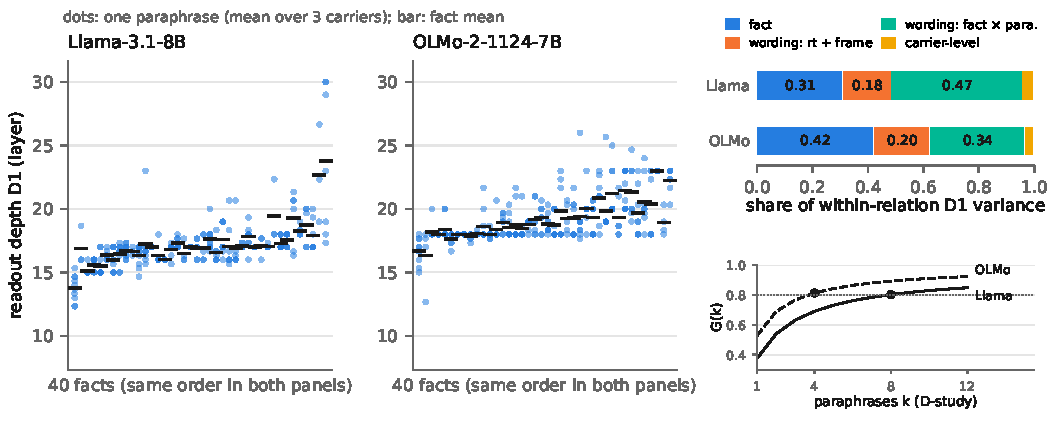
\includegraphics[width=\textwidth]{figs/fig1_p2.pdf}
\caption{\textbf{Readout depth of the same fact under different paraphrases (\STwo).}
\emph{Left, middle:} D1 in layers (of \ptNLayersLlama) for forty facts \emph{selected, not sampled}: two per relation with the most paraphrases correct in both models; correct cells only. Dots: paraphrases (mean over carriers); bars: fact means; same facts and order in both panels.
\emph{Right, top:} shares of within-relation D1 variance from the preregistered model (fact; paraphrase main effects; fact $\times$ paraphrase; carrier-level noise). The fact component includes answer-token identity. Splitting the paraphrase-related share is \expl; intervals are in Table~\ref{tab:p2}.
\emph{Right, bottom:} decision study, relative coefficient $G(k)$; dots mark \nprime{} for $G=\ptRuleG$ (estimation only).}
\label{fig:p2}
\end{figure*}

\section{Introduction}
Layer-wise measurements of factual recall are used to say where a model processes a fact: causal tracing and activation patching locate the layers that matter \citep{meng2022rome,geva2023dissecting}, lenses read out the answer at intermediate layers \citep{belrose2023tuned,ghandeharioun2024patchscopes}, and such depths are compared across facts and models \citep{gupta2025depth,hochman2026factual}.
These measurements are usually taken on one prompt per fact (\S\ref{sec:practice}).
A depth measured on one prompt is then read as a property of the fact, but it is also a property of the prompt.
Localisation is known to move with the phrasing of a query \citep{chen2024knowledge,benz2026knowledgedebugger}, and behaviour on the same fact varies across paraphrases and tasks \citep{elazar2021pararel,elhelo2026task}.
To our knowledge, no preregistered study has decomposed a layer-wise depth into fact-level and paraphrase-related variance.

We do this for one well-defined depth: the layer at which a model's answer becomes readable at the prediction position.
We patch the prompt's final-token hidden state at each layer into the final token of neutral carrier prompts and record when the probability of the object's first token reaches and keeps half its final value (\S\ref{sec:measure}).
This is a depth of answer readout; it says nothing about where a fact is stored or about the subject position.

We report two studies with frozen analysis plans, decision rules and wording rules (Appendix~\ref{app:integrity}).
\textbf{\SOne} (\S\ref{sec:hr}) tests whether depth depends on the relation or on pretraining co-occurrence, using exact subject--object counts.
\textbf{\STwo} (\S\ref{sec:p2}) measures facts under \ptNFrames{} designed paraphrases and decomposes depth variance.
Our contributions:
\begin{itemize}
\item An equivalence-bounded co-occurrence result: on all prompts of three models, within-relation co-occurrence changed the marginal \Rsq of depth by point estimates of at most \hrDRsqMax{} with upper bounds below \hrThrDRsqHi{} (not blind), and a preregistered test that relation identity carries a large share of depth failed in all three models.
\item A preregistered variance decomposition of readout depth over facts and paraphrases in two families, on correct prompts: the fact share, which includes answer-token identity, is above zero (estimates \ptIccRangeLo--\ptIccRangeHi), with paraphrase-related shares of \ptWordingRangeLo--\ptWordingRangeHi.
\item A decision study \citep{brennan2001gtheory} estimating how many paraphrases give a generalizability coefficient of \ptRuleG, a methods note on why patching depths are conditioned on correctness, and a complete record of preregistered tests, deviations and integrity incidents.
\end{itemize}

\section{Related work}
\label{sec:related}
\paragraph{Localisation and its limits.}
Causal tracing locates factual associations in middle-layer MLPs \citep{meng2022rome}, but localisation does not predict which layer is best to edit \citep{hase2023localization}.
\citet{chen2024knowledge} find that knowledge neurons are tied to the query rather than the fact for many ParaRel facts.
\citet{benz2026knowledgedebugger} show causal tracing placing one fact at different layers under three phrasings.
\citet{elhelo2026task} find task-specific encoding of facts, using ten paraphrases per dataset--task pair and a variance decomposition of behaviour; \citet{saynova2024scenarios} show that tracing results differ across prediction scenarios.
Prompt dependence is therefore not new; we quantify it for a readout depth, with preregistered tests and a decision study.
\paragraph{Depth, retrieval paths and reliability.}
\citet{gupta2025depth} find that the first token of a multi-token answer needs more depth; we control answer length as a covariate.
\citet{hochman2026factual} find retrieval to be redundant and non-contiguous, with per-relation path lengths that differ between models (no statistic reported); \citet{agarwal2026relation} find relation information active before entity information across prompt families; \citet{rohweder2026predicting} find that linear relational decodability depends mostly on the subject's representation.
\citet{meloux2025circuits} treat circuit discovery as statistical estimation with high variance under small input changes; we borrow reliability tools from generalizability theory \citep{brennan2001gtheory}.
\paragraph{Frequency and knowledge.}
Pretraining frequency predicts factual accuracy \citep{kandpal2023longtail,mallen2023popqa} and few-shot numerical reasoning \citep{razeghi2022frequencies}, and co-occurrence relates to the formation of linear relation representations \citep{merullo2025linear,hernandez2024linearity}.
\citet{bajpai2024popular}, using Wikipedia page views as popularity, report earlier convergence of internal states for popular questions in Llama-2 and paraphrase variability that grows with popularity; our counts are exact co-occurrences in the models' corpora \citep{liu2024infinigram}, and our depth is a patched readout.
Knowledge probing \citep{petroni2019lama} and its consistency across paraphrases \citep{elazar2021pararel} are long studied; \citet{dong2023karr} assess knowledge statistically over paraphrased prompts.
\paragraph{Preregistration.}
Preregistration has been proposed and debated for NLP \citep{vanmiltenburg2021prereg,sogaard2023prereg}, following practice elsewhere \citep{nosek2018prereg}.

\section{Measuring readout depth}
\label{sec:measure}
\subsection{Patch and outcomes}
For a fact prompt (e.g.\ ``Betiana Blum is a citizen of''), we take the residual stream at its final token after block $l$ and write it into the final token of each of three carriers, ``X is associated with'', ``X is linked to'' and ``A word that goes with X is'', where X is the literal letter, not the subject \citep{zhang2024patching,heimersheim2024patching}.
We run each carrier forward from block $l$ and record $p_c(l)$, the probability of the object's first token at the carrier's final position.
The primary depth D1 is the half-probability onset, normalised by the number of layers $L$:
\begin{align}
l^{*}_c&=\min\{l : p_c(l') \ge \tfrac{1}{2}\,p_c(L-1)\ \forall\, l' \ge l\}, \\ % allow-number (definition)
D1_c&=(l^{*}_c+1)/L. % allow-number (definition)
\end{align}
D4, a preregistered robustness outcome, is $1-\tfrac{1}{L}\sum_l \min(1, p_c(l)/p_c(L-1))$; both come from the same curve. % allow-number (definition)
Secondary outcomes are a stable $p \ge$ 0.1 onset and a stable rank-1 onset. % allow-number (outcome definition)

\subsection{Rank-based depth is conditioned on correctness}
\label{sec:audit}
\begin{figure}[t]
\centering
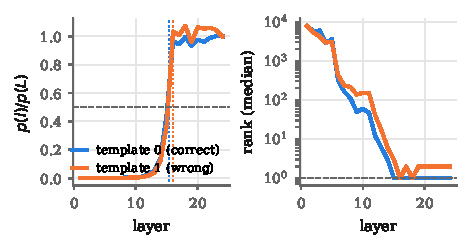
\includegraphics[width=\columnwidth]{figs/fig3_audit.pdf}
\caption{Worked example (\expl), \PythiaOneFourB: Weimar Republic $\to$ Berlin under two templates. Left: carrier-mean patched probability relative to its final value; dotted lines mark D1. Right: median rank of ``Berlin''. Only the correct prompt has a rank-1 onset; both have a D1.}
\label{fig:audit}
\end{figure}
A common alternative to D1 is the first layer from which the object is the top-ranked token at every later layer.
Under the final-token patch this depth exists only for correctly answered prompts.
At the last block the patched state is the source prompt's own final residual, so the carrier's output distribution equals the source's, and ``rank one at every layer up to the last'' requires rank one at the last layer, i.e.\ a correct answer.
Every prompt without a rank-1 depth is therefore a wrong one, and a censoring model of rank-1 depth models correctness, not timing.

Figure~\ref{fig:audit} shows one fact in \PythiaOneFourB{} (\expl worked example).
``The capital of Weimar Republic is'' is answered correctly: D1 falls at about layer \explAuditExDOneCorr{} of \explAuditExL{}, and ``Berlin'' is rank one from layer \explAuditExRankOnset{} on.
``The capital city of Weimar Republic is'' is answered wrongly (``Berlin'' ends at rank two): its D1 is about layer \explAuditExDOneWrong, but it has no rank-1 depth.
An audit of all rows confirms the derivation (\expl): in \PythiaOneFourB, \explAuditResCorrPyOneFour{} prompts resolved and were correct, \explAuditResWrongPyOneFour{} resolved and were wrong, \explAuditCensCorrPyOneFour{} were censored and correct and \explAuditCensWrongPyOneFour{} censored and wrong (\PythiaTwoEightB: \explAuditResCorrPyTwoEight, \explAuditResWrongPyTwoEight, \explAuditCensCorrPyTwoEight, \explAuditCensWrongPyTwoEight).
D1 is defined on wrong prompts too, but there it times half of a small final probability of the gold object.
\STwo therefore analyses correct cells, with all cells as a sensitivity; \SOne, frozen earlier, uses all rows.

\subsection{Measurement properties (\expl)}
\label{sec:props}
D1 is coarse: on \STwo's correct cells it takes \explNDistinctLlama{} distinct values in \llama{} and \explNDistinctOlmo{} in \olmo, and \explModalShareLlama{} and \explModalShareOlmo{} of cells sit at the modal layer (\explModalLayerLlama{} and \explModalLayerOlmo).
Its agreement with a logit-lens onset on \SOne's correct rows is weak: Spearman \explHrLensRhoPyOneFour, \explHrLensRhoPyTwoEight{} and \explHrLensRhoOlmoSeven{} (\explHrLensNPyOneFour, \explHrLensNPyTwoEight{} and \explHrLensNOlmoSeven{} rows).
Patching into carriers and decoding the residual directly therefore time different events, and our shares are specific to D1 and D4.

\section{\SOne: relation and co-occurrence}
\label{sec:hr}
\paragraph{Design.}
\PythiaOneFourB, \PythiaTwoEightB{} \citep{biderman2023pythia} and \olmo{} \citep{olmo2025two}; \hrNFacts{} facts (\hrNRelations{} relations $\times$ \hrNPerRelation) from CounterFact, PopQA and LRE \citep{meng2022rome,mallen2023popqa,hernandez2024linearity}, three templates each, all rows: only \hrNCorrectPyOneFour, \hrNCorrectPyTwoEight{} and \hrNCorrectOlmoSeven{} of \hrNPyOneFour{} rows per model are answered correctly.
Co-occurrence counts are EXACT phrase co-occurrences in each model's pretraining corpus (the Pile; OLMo-2's stage-1 mix, which excludes its mid-training data), counted with infini-gram \citep{liu2024infinigram}.
The preregistered model is a linear mixed model of D1 with five fact covariates (answer and subject token counts, the object's log-prior on generic prefixes, its final log-probability, subject-to-final distance) and random intercepts for relation, relation $\times$ template and subject \citep{bates2015lme4}.
\textbf{H1}: the adjusted relation share $\mathrm{ICC}_{rel} \ge \hrThrIcc$ with relation-cluster bootstrap lower bound $\ge \hrThrIccLo$ in every model.
\textbf{H2}: relation orderings agree across families (Spearman $\rho \ge \hrThrRho$, permutation $p<\hrThrPermP$; and a covariate-controlled version).
\textbf{H3}: adding within-relation (relation-centred) log co-occurrence changes the marginal \Rsq \citep{nakagawa2013r2} by less than \hrThrDRsqHi{} at the upper \ptCiLevel\% bound in every model.
\paragraph{Results.}
H1 failed in all three models (Table~\ref{tab:hr}, Figure~\ref{fig:hr}): the relation share was \hrIccPyOneFour, \hrIccPyTwoEight{} and \hrIccOlmoSeven, with upper bounds of \hrIccHiPyOneFour, \hrIccHiPyTwoEight{} and \hrIccHiOlmoSeven.
A failed positive test is not a confirmed null, and the relation effect is template-specific: relation $\times$ template carried \explHrShareRtPyOneFour, \explHrShareRtPyTwoEight{} and \explHrShareRtOlmoSeven{} of the random variance (\expl breakdown), and in the preregistered non-gating variants the relation share was \hrIccTemplateMin--\hrIccTemplateMax{} when each template is fitted alone and \hrIccCorrectOnlyMin--\hrIccCorrectOnlyMax{} on correct rows only (Appendix~\ref{app:hrvar}).
This template dependence is the same prompt dependence that \STwo measures.
Relation orderings were shared across families at $\rho=\hrRhoPyOneFourOlmo$ and \hrRhoPyTwoEightOlmo{} (one-sided permutation $p=\hrPermPPyOneFourOlmo$ and \hrPermPPyTwoEightOlmo): above chance, below the H2 threshold; the controlled version also failed.
H3 passed in all three models: \DRsq{} was \hrDRsqPyOneFour, \hrDRsqPyTwoEight{} and \hrDRsqOlmoSeven, with upper bounds \hrDRsqHiPyOneFour, \hrDRsqHiPyTwoEight{} and \hrDRsqHiOlmoSeven.
The frozen decision rule gives \hrDecision{} for a relation-driven account of depth.

Four qualifications.
(i)~H3 was not blind: an earlier analysis of the same rows had shown a small effect, disclosed in the prereg.
(ii)~The model conditions on the final log-probability, which co-occurrence also predicts (correctness odds ratio per unit of log co-occurrence \hrOrPyOneFour, \hrOrPyTwoEight, \hrOrOlmoSeven), so H3 bounds the association given confidence.
(iii)~The co-occurrence coefficient itself is clearly non-zero but small (\expl, in layers per unit of log co-occurrence): \explHrSlopePyOneFour{} \ci{\explHrSlopeLoPyOneFour}{\explHrSlopeHiPyOneFour}, \explHrSlopePyTwoEight{} \ci{\explHrSlopeLoPyTwoEight}{\explHrSlopeHiPyTwoEight} and \explHrSlopeOlmoSeven{} \ci{\explHrSlopeLoOlmoSeven}{\explHrSlopeHiOlmoSeven}.
(iv)~A non-gating discrete-time survival model with relation frailty only gives hazard ratios per unit of log co-occurrence of \hrSurvHrPyOneFour{} \ci{\hrSurvHrLoPyOneFour}{\hrSurvHrHiPyOneFour}, \hrSurvHrPyTwoEight{} and \hrSurvHrOlmoSeven, i.e.\ slightly later readout with more co-occurrence; its Wald $p$-values ignore clustering by fact and template and are anti-conservative.
Most rows are wrong answers, for which D1 has a different meaning (\S\ref{sec:audit}); the correct-only variant gives \DRsq{} of \hrDRsqCorrectOnlyPyOneFour, \hrDRsqCorrectOnlyPyTwoEight{} and \hrDRsqCorrectOnlyOlmoSeven{} without intervals.

\begin{table}[t]
\centering\small
\setlength{\tabcolsep}{3pt} % allow-number (layout)
\resizebox{\columnwidth}{!}{%
\begin{tabular}{@{}lccc@{}}
\toprule
 & \PythiaOneFourB & \PythiaTwoEightB & OLMo-2-7B \\
\midrule
rows / correct & \hrNPyOneFour{} / \hrNCorrectPyOneFour & \hrNPyTwoEight{} / \hrNCorrectPyTwoEight & \hrNOlmoSeven{} / \hrNCorrectOlmoSeven \\
$\mathrm{ICC}_{rel}$ & \hrIccPyOneFour & \hrIccPyTwoEight & \hrIccOlmoSeven \\
\quad CI & \ci{\hrIccLoPyOneFour}{\hrIccHiPyOneFour} & \ci{\hrIccLoPyTwoEight}{\hrIccHiPyTwoEight} & \ci{\hrIccLoOlmoSeven}{\hrIccHiOlmoSeven} \\
H1 & \hrHOnePassPyOneFour & \hrHOnePassPyTwoEight & \hrHOnePassOlmoSeven \\
\DRsq & \hrDRsqPyOneFour & \hrDRsqPyTwoEight & \hrDRsqOlmoSeven \\
\quad CI & \ci{\hrDRsqLoPyOneFour}{\hrDRsqHiPyOneFour} & \ci{\hrDRsqLoPyTwoEight}{\hrDRsqHiPyTwoEight} & \ci{\hrDRsqLoOlmoSeven}{\hrDRsqHiOlmoSeven} \\
H3 & \hrHThreePassPyOneFour & \hrHThreePassPyTwoEight & \hrHThreePassOlmoSeven \\
survival HR & \hrSurvHrPyOneFour & \hrSurvHrPyTwoEight & \hrSurvHrOlmoSeven \\
correct OR & \hrOrPyOneFour & \hrOrPyTwoEight & \hrOrOlmoSeven \\
\midrule
 & \multicolumn{2}{c}{vs.\ OLMo (cross-family)} & \\ % allow-number (layout)
H2 $\rho$ & \hrRhoPyOneFourOlmo & \hrRhoPyTwoEightOlmo & \\
\quad perm.\ $p$ & \hrPermPPyOneFourOlmo & \hrPermPPyTwoEightOlmo & \\
partial $\rho$ & \hrPRhoPyOneFourOlmo & \hrPRhoPyTwoEightOlmo & \\
H2 raw / ctl. & \hrHTwoRawPassPyOneFourOlmo{} / \hrHTwoCtlPassPyOneFourOlmo & \hrHTwoRawPassPyTwoEightOlmo{} / \hrHTwoCtlPassPyTwoEightOlmo & \\
\bottomrule
\end{tabular}}
\caption{\SOne (H-R prereg), all rows. \ptCiLevel\% relation-cluster bootstrap intervals (\hrNBootRel{} resamples). HR: survival hazard ratio per log co-occurrence (non-gating). OR: correctness odds ratio. Decision: \hrDecision.}
\label{tab:hr}
\end{table}

\begin{figure}[t]
\centering
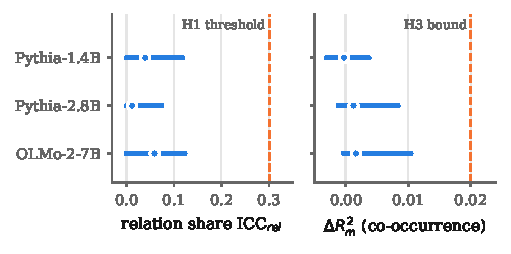
\includegraphics[width=\columnwidth]{figs/fig2_hr_forest.pdf}
\caption{\SOne, all rows (\hrNPyOneFour{} per model). Left: adjusted relation share against the H1 threshold. Right: change in marginal \Rsq from within-relation co-occurrence against the H3 bound. Bars: \ptCiLevel\% relation-cluster bootstrap intervals.}
\label{fig:hr}
\end{figure}

\section{\STwo: fact versus paraphrase}
\label{sec:p2}
\subsection{Design}
\begin{table*}[t]
\centering\footnotesize\setlength{\tabcolsep}{3pt} % allow-number (layout)
\begin{tabular}{@{}ll@{}}
\toprule
frame & template (relation: citizenship) \\
\midrule
\texttt{SF-cloze-short} & X is a citizen of \\
\texttt{SF-cloze-long} & According to reference sources, X is a citizen of \\
\texttt{RF-cloze-short} & The country of citizenship of X is \\
\texttt{RF-cloze-long} & According to reference sources, the country of citizenship of X is \\
\texttt{SF-question-short} & Q: X is a citizen of which country? $\hookleftarrow$ A: \\
\texttt{SF-question-long} & Q: According to reference sources, X is a citizen of which country? $\hookleftarrow$ A: \\
\texttt{RF-question-short} & Q: Which country is X a citizen of? $\hookleftarrow$ A: \\
\texttt{RF-question-long} & Q: According to reference sources, which country is X a citizen of? $\hookleftarrow$ A: \\
\texttt{LEX1-SF-cloze-short} & X holds citizenship of \\
\texttt{LEX2-RF-cloze-short} & The country whose citizenship X holds is \\
\bottomrule
\end{tabular}
\caption{The designed frames for one relation (SF/RF: subject-first / relation-first). Every relation has the same frame types.}
\label{tab:frames}
\end{table*}
\paragraph{Materials and prior exposure.}
\ptNFacts{} facts over \ptNRelations{} relations (mostly CounterFact; Appendix~\ref{app:data}), sampled five per co-occurrence tercile per relation, each phrased with \ptNFrames{} designed frames (Table~\ref{tab:frames}): subject-first vs.\ relation-first order, cloze vs.\ question form, short vs.\ long (a neutral prefix), plus two lexical variants.
The plan was written after \SOne and after an earlier \expl decomposition on three templates, which had found within-relation fact shares of \ptPriorIccLo--\ptPriorIccHi{} and one OLMo result that depended on a single relation (difference \ptPriorCeoBefore{} with it, \ptPriorCeoAfter{} without); that relation fails the sampling rule and is not in \STwo, and \ptPriorOverlap{} of the \ptNFacts{} facts were seen before.
\paragraph{Models and inclusion.}
\ptNPreregModels{} preregistered models from four families (\QwenThreeEightB, \llama, \PythiaOneFourB, \PythiaTwoEightB, \olmo; \citealp{yang2025qwen3,grattafiori2024llama}), run once in fp32 with all \ptNFacts{} $\times$ \ptNFrames{} cells and \ptNcUsed{} carriers.
A cell is correct if the top-1 next token is the object's first token.
A model is included only if at least \ptRuleMinFacts{} facts have at least \ptRuleMinCorrect{} correct paraphrases, covering at least \ptRuleMinRel{} relations: \llama{} (\ptIncFactsLlama{} such facts) and \olmo{} (\ptIncFactsOlmo) were included; \QwenThreeEightB{} (\ptIncFactsQwen), \PythiaOneFourB{} (\ptIncFactsPyOneFour) and \PythiaTwoEightB{} (\ptIncFactsPyTwoEight) are MISSING (insufficient data).
The fit then uses every correct cell, including facts with a single correct paraphrase: \ptNCellsLlama{} cells of \ptNFactsLlama{} facts and \ptNCellsOlmo{} of \ptNFactsOlmo.
\paragraph{Model.}
D1 is modelled on carrier-level rows by REML with four fact covariates (answer and subject token counts; the answer's prior on the carriers alone; log co-occurrence, a PROXY count from DCLM-baseline \citep{li2024dclm} for both models) and a carrier fixed effect:
\begin{align*}
y \sim{}& \text{covariates} + \text{carrier} + (1|\text{rel}) + (1|\text{frame}) \\ % allow-number (formula notation)
&+ (1|\text{rel}{:}\text{frame}) + (1|\text{fact}) \\ % allow-number (formula notation)
&+ (1|\text{fact}{:}\text{frame}) + (1|\text{fact}{:}\text{carrier}). % allow-number (formula notation)
\end{align*}
Let the within-relation variance of a carrier-averaged depth be the sum of the fact, relation $\times$ frame, frame and fact $\times$ frame components plus the fact $\times$ carrier and residual components divided by the number of carriers.
The \textbf{fact share} (written \ICCone) is the fact component over this sum; the \textbf{paraphrase-related share} is the frame, relation $\times$ frame and fact $\times$ frame components over the sum.
Both are conditional on the covariates and are not the Shrout--Fleiss ICC.
Intervals are parametric bootstrap percentile intervals (\ptNBoot{} resamples), the method chosen by a preregistered simulation (Appendix~\ref{app:sims}).
\paragraph{Tests.}
\textbf{H1} (paraphrase $>$ fact): the paraphrase-related share minus \ICCone{} has a \ptCiLevel\% interval above zero under D1 and D4, and a method-of-moments (MoM) estimate agrees in sign.
\textbf{H1-alt} (fact-dominated): \ICCone{} $\ge \ptRuleAltIcc$ with lower bound $\ge \ptRuleAltIccLo$ under D1 and D4, and MoM difference below zero.
\textbf{Fact-share null}: a parametric bootstrap with fact variance set to zero and all other components as estimated (\ptRuleNBootNull{} datasets); ``the fact share is above zero'' requires $p<\ptRuleNullP$.
Each headline sentence needs its condition in at least \ptRuleMinFamilies{} families (Table~\ref{tab:rules}).
\textbf{H2} and \textbf{H3} are estimates: \ICCone, \nprime{} (the number of paraphrases for a relative coefficient $G(k) \ge \ptRuleG$) and the cross-model correlation of fact means.

\subsection{Results}
\begin{table}[t]
\centering\small
\setlength{\tabcolsep}{4pt} % allow-number (layout)
\resizebox{\columnwidth}{!}{%
\begin{tabular}{@{}lcc@{}}
\toprule
 & \llama & OLMo-2-7B \\
\midrule
facts / cells & \ptNFactsLlama{} / \ptNCellsLlama & \ptNFactsOlmo{} / \ptNCellsOlmo \\
\ICCone, D1 & \ptIccDOneLlama{} \ci{\ptIccDOneLoLlama}{\ptIccDOneHiLlama} & \ptIccDOneOlmo{} \ci{\ptIccDOneLoOlmo}{\ptIccDOneHiOlmo} \\
\ICCone, D4 & \ptIccDFourLlama{} \ci{\ptIccDFourLoLlama}{\ptIccDFourHiLlama} & \ptIccDFourOlmo{} \ci{\ptIccDFourLoOlmo}{\ptIccDFourHiOlmo} \\
paraphrase, D1 & \ptWordingDOneLlama{} \ci{\ptWordingDOneLoLlama}{\ptWordingDOneHiLlama} & \ptWordingDOneOlmo{} \ci{\ptWordingDOneLoOlmo}{\ptWordingDOneHiOlmo} \\
paraphrase, D4 & \ptWordingDFourLlama{} \ci{\ptWordingDFourLoLlama}{\ptWordingDFourHiLlama} & \ptWordingDFourOlmo{} \ci{\ptWordingDFourLoOlmo}{\ptWordingDFourHiOlmo} \\
diff, D1 & \ptDiffDOneLlama{} \ci{\ptDiffDOneLoLlama}{\ptDiffDOneHiLlama} & \ptDiffDOneOlmo{} \ci{\ptDiffDOneLoOlmo}{\ptDiffDOneHiOlmo} \\
diff, D4 & \ptDiffDFourLlama{} \ci{\ptDiffDFourLoLlama}{\ptDiffDFourHiLlama} & \ptDiffDFourOlmo{} \ci{\ptDiffDFourLoOlmo}{\ptDiffDFourHiOlmo} \\
MoM diff D1 / D4 & \ptMomDiffDOneLlama{} / \ptMomDiffDFourLlama & \ptMomDiffDOneOlmo{} / \ptMomDiffDFourOlmo \\
H1 / H1-alt & \ptHOneLlama{} / \ptHOneAltLlama & \ptHOneOlmo{} / \ptHOneAltOlmo \\
null $p$ (null upper pct.) & \ptNullPLlama{} (\ptNullNinetyNineLlama) & \ptNullPOlmo{} (\ptNullNinetyNineOlmo) \\
\nprime{} for $G=\ptRuleG$ & \ptNprimeLlama{} \ci{\ptNprimeLoLlama}{\ptNprimeHiLlama} & \ptNprimeOlmo{} \ci{\ptNprimeLoOlmo}{\ptNprimeHiOlmo} \\
$G$ ceiling & \ptGCeilLlama & \ptGCeilOlmo \\
\midrule
\multicolumn{3}{@{}l@{}}{\QwenThreeEightB, \PythiaOneFourB, \PythiaTwoEightB: MISSING (insufficient data)} \\ % allow-number (layout)
\bottomrule
\end{tabular}}
\caption{\STwo (P2 prereg), correct cells. Shares are within relation; diff $=$ paraphrase-related share $-$ \ICCone. \ptCiLevel\% parametric bootstrap intervals (\ptNBoot{} resamples). Null: \ptRuleNBootNull{} datasets; $p$ equals its floor; the bracket gives the null distribution's upper percentile at $p=\ptRuleNullP$.}
\label{tab:p2}
\end{table}

\begin{table}[t]
\centering\small
\resizebox{\columnwidth}{!}{%
\begin{tabular}{@{}ll@{}}
\toprule
preregistered headline sentence (condition) & outcome \\
\midrule
``The fact share is above zero'' (null $p<\ptRuleNullP$) & \ptClaimFactShare \\
``There is no fixed layer where a fact lives'' (\ICCone{} upper $<\ptRuleNoFixedHi$) & \ptClaimNoFixedLayer \\
``A single prompt is a poor estimate \dots; it takes N paraphrases'' (H1, \nprime{} $\ge \ptRuleNprimeMin$) & \ptClaimSinglePromptPoor \\
``Wording shifts every fact's depth together'' (H1, systematic $>$ residual) & \ptClaimWordingTogether \\
``Facts have a depth that frequency and relation do not explain'' (H1-alt) & \ptClaimFactUnexplained \\
model-dependent (H1 and H1-alt each in $\ge \ptRuleMinFamilies$ families) & \ptClaimModelDep \\
\bottomrule
\end{tabular}}
\caption{\STwo headline wording rules (each condition in at least \ptRuleMinFamilies{} families) and their outcomes. Only the first sentence is licensed.}
\label{tab:rules}
\end{table}

\begin{table}[t]
\centering\small
\resizebox{\columnwidth}{!}{% GENERATED by scripts/make_tables.py; do not edit.
\begin{tabular}{@{}lrrrrr@{}}
\toprule
model, outcome & fact (frozen) & fact (+object) & object & fact (+log-prob) & fact (+both) \\
\midrule
\llama, D1 & \explObjBaseDOneLlama & \explObjFactDOneLlama & \explObjObjDOneLlama & \explLpFactDOneLlama & \explObjLpFactDOneLlama \\
OLMo-2-7B, D1 & \explObjBaseDOneOlmo & \explObjFactDOneOlmo & \explObjObjDOneOlmo & \explLpFactDOneOlmo & \explObjLpFactDOneOlmo \\
\llama, D4 & \explObjBaseDFourLlama & \explObjFactDFourLlama & \explObjObjDFourLlama & \explLpFactDFourLlama & \explObjLpFactDFourLlama \\
OLMo-2-7B, D4 & \explObjBaseDFourOlmo & \explObjFactDFourOlmo & \explObjObjDFourOlmo & \explLpFactDFourOlmo & \explObjLpFactDFourOlmo \\
\bottomrule
\end{tabular}
}
\caption{\expl refits of the frozen \STwo model (point estimates, correct cells): fact share as preregistered, with a relation $\times$ object term, the object share, and with the cell-level final log-probability as a covariate.}
\label{tab:obj}
\end{table}

\paragraph{The fact share is above zero.}
This is the one headline sentence the preregistration licenses (Table~\ref{tab:rules}; null $p$ at its floor in both families, observed \ICCone{} at least \ptNullRatioMin{} times the largest null value).
It was expected: the earlier exploratory decomposition had found fact shares of \ptPriorIccLo--\ptPriorIccHi, so the test works more as a check than as a discovery.
It means that fact-level variance, which includes the identity of the answer token and anything else constant within a fact, is above zero; it does not say that facts have their own depth.
An \expl refit that adds a relation $\times$ object term (\explNObjectsLlama{} and \explNObjectsOlmo{} distinct answers) splits the fact component: the remaining fact share is \explObjFactDOneLlama{} (\llama) and \explObjFactDOneOlmo{} (\olmo) under D1, with \explObjObjDOneLlama{} and \explObjObjDOneOlmo{} attributed to the answer (Table~\ref{tab:obj}); adding the unpatched prompt's final log-probability as a cell-level covariate changes little (\explObjLpFactDOneLlama{} and \explObjLpFactDOneOlmo{} with both terms).
Llama and OLMo also share first-token ids for the objects, so token-driven variance is not independent across the two families.

\paragraph{Paraphrase-related variance.}
The paraphrase-related share was \ptWordingDOneLlama{} and \ptWordingDOneOlmo{} under D1 (\ptWordingDFourLlama{} and \ptWordingDFourOlmo{} under D4).
H1 held in \llama{} and not in \olmo, whose D1 difference interval reaches \ptDiffDOneLoOlmo, so no family-level sentence about wording is licensed (\ptNFamiliesHOne{} of \ptNFamiliesIncluded{} families); \olmo{} passes H1 in three non-gating sensitivity sets, so its failure is narrow.
We treat the \llama{} result as weak: in our robustness simulation the single-measure interval condition passed in \ptRobDiffLoPosMin--\ptRobDiffLoPosMax{} of datasets with a true difference of zero (nominal \ptNominalOneSided) and the difference was biased upward (\S\ref{sec:robust}); \llama's lower bound of \ptDiffDOneLoLlama{} is, however, far from zero.
H1-alt held in neither model.

\begin{table}[t]
\centering\small
\resizebox{\columnwidth}{!}{% GENERATED by scripts/make_tables.py; do not edit.
\begin{tabular}{@{}lrr@{}}
\toprule
change within a fact (layers) & \llama & OLMo-2-7B \\
\midrule
add neutral prefix (long vs short) & \explPairPrefixLlama (\explPairPrefixNLlama) & \explPairPrefixOlmo (\explPairPrefixNOlmo) \\
subject-first vs relation-first & \explPairOrderLlama (\explPairOrderNLlama) & \explPairOrderOlmo (\explPairOrderNOlmo) \\
cloze vs question & \explPairFormLlama (\explPairFormNLlama) & \explPairFormOlmo (\explPairFormNOlmo) \\
lexical variant & \explPairLexicalLlama (\explPairLexicalNLlama) & \explPairLexicalOlmo (\explPairLexicalNOlmo) \\
\midrule
mean shift: relation-first $-$ subject-first & \explHFourOrderLlama & \explHFourOrderOlmo \\
mean shift: question $-$ cloze & \explHFourFormLlama & \explHFourFormOlmo \\
mean shift: long $-$ short & \explHFourLengthLlama & \explHFourLengthOlmo \\
range of the ten frame means & \explHFourRangeLlama & \explHFourRangeOlmo \\
\bottomrule
\end{tabular}
}
\caption{\expl What moves D1 (layers, correct cells). Top: root-mean-square change within a fact between two frames that differ in one feature (number of fact--frame pairs). Bottom: preregistered \expl H4 frame effects (fixed-effect refit), average shifts.}
\label{tab:pairs}
\end{table}

What is the paraphrase-related variance made of (\expl)?
Under D1 the fact $\times$ paraphrase share was \explFtShareLlama{} and \explFtShareOlmo, against \explSysWordShareLlama{} and \explSysWordShareOlmo{} for paraphrase main effects, but under D4 the split is \explDFourFtLlama{} vs.\ \explDFourSysLlama{} and \explDFourFtOlmo{} vs.\ \explDFourSysOlmo, so which part dominates depends on the measure.
The preregistered ``shifts together'' quantity was negative under D1 (\ptTfResidLlama, \ptTfResidOlmo).
Small edits move depth as much as large ones (Table~\ref{tab:pairs}): within a fact, adding only the neutral prefix ``According to reference sources,'' changes D1 by \explPairPrefixLlama{} and \explPairPrefixOlmo{} layers (root mean square), similar to changing order (\explPairOrderLlama, \explPairOrderOlmo), form (\explPairFormLlama, \explPairFormOlmo) or a lexical variant (\explPairLexicalLlama, \explPairLexicalOlmo).
The preregistered \expl frame effects (H4) are small on average: relation-first frames are read out \explHFourOrderLlama{} and \explHFourOrderOlmo{} layers relative to subject-first ones, questions \explHFourFormLlama{} and \explHFourFormOlmo{} relative to cloze, long frames \explHFourLengthLlama{} and \explHFourLengthOlmo{} relative to short, and all frame means lie within \explHFourRangeLlama{} and \explHFourRangeOlmo{} layers.
The paraphrase-related variance is thus mostly sensitivity of individual facts to any small change of the prompt, not a few systematic frame effects. For scale, the fact effects have a standard deviation of \explSdFactLayersLlama{} and \explSdFactLayersOlmo{} layers (\expl).

\paragraph{Agreement across models.}
For the \ptHThreeN{} facts analysed in both models, fact-mean depths correlate at $\rho=\ptHThreeRho$, and \ptHThreeDisatt{} after approximate disattenuation by each model's coefficient for its mean number of correct paraphrases (\ptHThreeKbarLlama{} and \ptHThreeKbarOlmo).
This estimate is limited to correct cells, D1 and shared answer tokens.

\paragraph{Decision study.}
For a relative coefficient of \ptRuleG{} (the fact's depth relative to other facts of its relation), the estimated number of paraphrases per fact is \ptNprimeLlama{} \ci{\ptNprimeLoLlama}{\ptNprimeHiLlama} for \llama{} and \ptNprimeOlmo{} \ci{\ptNprimeLoOlmo}{\ptNprimeHiOlmo} for \olmo{} (estimation only; same exchangeable paraphrases for every fact).
The estimate depends on the coefficient and the measure (\expl): the absolute coefficient, which also counts frame effects, needs \explNprimePhiDOneLlama{} and \explNprimePhiDOneOlmo{} paraphrases under D1, and the relative one needs \explNprimeGDFourLlama{} and \explNprimeGDFourOlmo{} under D4.
It counts correct paraphrases, and only \explFactsGeEightLlama{} of \ptNFactsLlama{} \llama{} facts and \explFactsGeEightOlmo{} of \ptNFactsOlmo{} \olmo{} facts have at least eight; selection on correctness makes these estimates optimistic.

\begin{table*}[t]
\centering\small
\setlength{\tabcolsep}{4pt} % allow-number (layout)
% GENERATED by scripts/make_tables.py; do not edit.
\begin{tabular}{@{}lrrrrrrrr@{}}
\toprule
 & \multicolumn{4}{c}{\llama} & \multicolumn{4}{c}{OLMo-2-7B} \\
\cmidrule(lr){2-5}\cmidrule(l){6-9}
set & facts & \ICCone & diff & lo & facts & \ICCone & diff & lo \\
\midrule
new facts only & \ptSensNewNFactsLlama & \ptSensNewIccDOneLlama & \ptSensNewDiffDOneLlama & \ptSensNewDiffDOneLoLlama & \ptSensNewNFactsOlmo & \ptSensNewIccDOneOlmo & \ptSensNewDiffDOneOlmo & \ptSensNewDiffDOneLoOlmo \\
all cells & \ptSensAllNFactsLlama & \ptSensAllIccDOneLlama & \ptSensAllDiffDOneLlama & \ptSensAllDiffDOneLoLlama & \ptSensAllNFactsOlmo & \ptSensAllIccDOneOlmo & \ptSensAllDiffDOneOlmo & \ptSensAllDiffDOneLoOlmo \\
correct under all frames & \ptSensAllTenNFactsLlama & \ptSensAllTenIccDOneLlama & \ptSensAllTenDiffDOneLlama & \ptSensAllTenDiffDOneLoLlama & \ptSensAllTenNFactsOlmo & \ptSensAllTenIccDOneOlmo & \ptSensAllTenDiffDOneOlmo & \ptSensAllTenDiffDOneLoOlmo \\
without manufacturer & \ptSensNoManuNFactsLlama & \ptSensNoManuIccDOneLlama & \ptSensNoManuDiffDOneLlama & \ptSensNoManuDiffDOneLoLlama & \ptSensNoManuNFactsOlmo & \ptSensNoManuIccDOneOlmo & \ptSensNoManuDiffDOneOlmo & \ptSensNoManuDiffDOneLoOlmo \\
template covariates & \ptSensTcovNFactsLlama & \ptSensTcovIccDOneLlama & \ptSensTcovDiffDOneLlama & \ptSensTcovDiffDOneLoLlama & \ptSensTcovNFactsOlmo & \ptSensTcovIccDOneOlmo & \ptSensTcovDiffDOneOlmo & \ptSensTcovDiffDOneLoOlmo \\
leave one frame out & -- & \ptLofoIccDOneMinLlama--\ptLofoIccDOneMaxLlama & \ptLofoDiffDOneMinLlama--\ptLofoDiffDOneMaxLlama & -- & -- & \ptLofoIccDOneMinOlmo--\ptLofoIccDOneMaxOlmo & \ptLofoDiffDOneMinOlmo--\ptLofoDiffDOneMaxOlmo & -- \\
\bottomrule
\end{tabular}

\caption{Preregistered \STwo sensitivities (D1; non-gating). lo: lower bound of the difference interval. Leave one frame out: range of point estimates over the ten frames.}
\label{tab:sens}
\end{table*}

\paragraph{Sensitivities.}
Preregistered sensitivities (non-gating) keep the D1 fact share between \ptSensIccDOneMin{} and \ptSensIccDOneMax{} across sets and models: the facts not seen before (\ptSensNewNFactsLlama{} and \ptSensNewNFactsOlmo{} facts), all cells, facts correct under all ten frames (only \ptSensAllTenNFactsLlama{} and \ptSensAllTenNFactsOlmo{} facts, which give the lowest values), without the manufacturer relation (the only influential relation in the sample), with template covariates, and leaving out one frame at a time (Table~\ref{tab:sens}).

\subsection{Robustness simulation (non-selecting)}
\label{sec:robust}
A preregistered simulation (\ptRobNSim{} datasets in each of eight conditions; frozen formula; D1 discretised to $L$ layers; missingness tied to late latent depth; two or three carriers; true difference zero) checked the intervals near the decision boundaries.
Coverage of \ICCone{} was \ptRobCovIccMin--\ptRobCovIccMax{} (nominal \ptCiLevel\%), with the truth above the interval in \ptRobIccMissAbove{} and below it in \ptRobIccMissBelow{} of \ptRobNTotal{} datasets, so the fact-share intervals err low; the licensed sentence itself rests on the null test, whose calibration is in Appendix~\ref{app:sims}.
The single-measure H1 interval condition was liberal, as above; the full H1 condition (D1, D4 and MoM together) was not simulated.
The simulation cannot change any decision.

\section{What this implies for single-prompt depths}
\label{sec:practice}
Published layer-wise analyses of factual recall typically use one prompt per fact.
\citet{meng2022rome} trace ``1000'' CounterFact facts, one text each: ``We use the text up to but not including the object [\dots] as the prompt, and we randomly sample 1000 of these texts'' (App.~B.1). % allow-number (quotation)
\citet{geva2023dissecting} build ``a data sample for each model, resulting in 1,209 queries for GPT-2 and 1,199 for GPT-J'', one query per triplet (\S3). % allow-number (quotation)
\citet{hochman2026factual} ``select 2,000 prompts for which the target attribute is a single token and this token is correctly predicted by the model'' (\S6). % allow-number (quotation)
These studies average over many facts, which is what their questions need, and our results do not bear on their conclusions.
They do bear on per-fact or per-relation readings of single-prompt depths.
For our depth measure, in our two models and on correct prompts, the relative generalizability of one prompt's depth, read from the preregistered $G(k)$ curve, is \explGOneLlama{} (\llama) and \explGOneOlmo{} (\olmo): roughly half or more of a single prompt's deviation from its relation (frame main effects excluded) does not carry over to other paraphrases of the same fact.
This is an estimate, not the preregistered sentence ``a single prompt is a poor estimate of a fact's depth'', whose condition was not met (Table~\ref{tab:rules}), and it does not transfer to other measures, positions or models.
A practical consequence within that scope: per-fact or per-relation depth comparisons with our measure should report how many paraphrases were averaged and how stable the ordering is across them.

\section{Discussion}
\paragraph{What the licensed sentence says.}
In \llama{} and \olmo, on correctly answered prompts, readout depth has a fact-level part that is above zero; part of it is the identity of the answer (\expl).
In both models the estimated paraphrase-related share is larger than the estimated fact share, with the difference confirmed by the preregistered test in one model only; most of that variance reflects how individual facts respond to small prompt changes (\expl).
\paragraph{\SOne in this light.}
The relation-level share was small on all rows pooled over templates, but large when each template was fitted alone; relation effects too are prompt-specific.
For frequency, the exact-count result bounds explained variance given confidence, not the association: the co-occurrence slope is non-zero but a fraction of a layer per unit of log co-occurrence.
\paragraph{Relation to prior work.}
That localisation moves with phrasing was shown anecdotally \citep{benz2026knowledgedebugger}, at neuron level \citep{chen2024knowledge} and for behaviour \citep{elhelo2026task}.
Our addition is a preregistered quantification for one readout depth, with a null test, an answer-identity check and a reliability estimate.

\section{Conclusion}
In \llama{} and \olmo, on correct prompts, the fact share of answer-readout depth is above zero, and about half of it is answer identity (\expl).
The estimated paraphrase-related share is larger, confirmed by the preregistered test in one of two models with a liberal test, and a separate study found that exact co-occurrence adds almost no explained variance given confidence.
Code, materials, curves and the preregistration record will be released (Appendix~\ref{app:data}).

\section*{Limitations}
\STwo includes two model families, which share answer first-token ids; three preregistered models answered too few facts under a first-token correctness criterion and are MISSING.
Both studies are English and use models of at most eight billion parameters.
\STwo analyses correct cells only; selection on correctness can bias the components and makes the decision study optimistic.
\SOne analyses all rows, most of them wrong answers, for which D1 times half of a small gold probability.
The depth is a readout at the final position under a final-token patch; it agrees weakly with a logit-lens onset, it is discrete with many cells at one layer, and we did not patch the subject position (future work).
The fact component includes answer-token identity; our relation $\times$ object refit is \expl.
The ten frames are designed, not sampled, so the shares describe variation over frames like these.
The co-occurrence covariate in \STwo is a PROXY count; \SOne's OLMo counts cover stage-1 pretraining only.
Both studies use Gaussian mixed models on a discrete outcome; \SOne's survival model ignores clustering by fact and template.
The CI method was chosen at a second look of a preregistered simulation; the robustness simulation shows under-coverage near the boundaries, and the fact-share null was mildly liberal in calibration with power \ptCalPowerRejOne{} at a fact share of a tenth (Appendix~\ref{app:sims}).
\SOne's H3 was not blind, and \STwo's plan was written after \SOne and an earlier exploratory decomposition were known.
The headline bootstrap intervals and the fact-share null were not independently recomputed by our replication agent (Appendix~\ref{app:integrity}).
A controlled-frequency pretraining experiment run on CPU learned too few facts to be informative and is not used.

\section*{Ethics statement}
We use public open-weight models under their licences and facts about public entities from public datasets; no personal data was collected and no human subjects were involved.
Release decisions follow each source's licence (Appendix~\ref{app:data}); where terms were unclear we release regeneration scripts instead of data.
Compute: GPU inference of about \cmpGpuMinHr{} minutes for \SOne{} and \cmpGpuMinPTwo{} minutes for \STwo{} (one GPU, fp32), and CPU for all analyses and simulations.
We see no specific misuse of readout-depth measurements beyond those of interpretability methods in general.

\section*{Acknowledgements}
\emph{AI assistance (disclosed per the ACL policy and Responsible NLP checklist item E1).}
The experiments, analysis code and drafting of this paper were done with Claude Code agents, working under the two preregistrations and a guard harness (frozen files, an append-only run ledger, generated numbers, independent review agents; Appendix~\ref{app:integrity}).
Claims were checked at human gates, the last before submission included.
The human author is responsible for all content.
AI tools are not authors.
Further acknowledgements are withheld for review.

\bibliography{refs}

\appendix
% Appendix (G5 draft). Numbers via numbers.tex macros; long tables are generated (paper/generated/, scripts/make_tables.py).
\FloatBarrier
\section{Integrity record}
\label{app:integrity}
This appendix lists what was fixed in advance, every departure from it, every integrity incident, the guards that enforce the rules, and every review.
All entries are generated from the project repository (\texttt{scripts/integrity\_summary.py}, run through the run ledger); the repository will be released with the paper.

\subsection{Preregistrations}
\begin{table*}[h]
\centering\small
\begin{tabular}{@{}llll@{}}
\toprule
study & file & frozen at & sha256 (prefix) \\
\midrule
\SOne (H-R) & \texttt{HR\_revised.md} & commit \texttt{\intHrCommit} & \texttt{\intHrSha} \\
\STwo (P2) & \texttt{P2\_prompt\_vs\_fact.md} & tag \texttt{prereg-P2} (\texttt{\intPtCommit}) & \texttt{\intPtSha} \\
\bottomrule
\end{tabular}
\caption{Preregistrations. Both files are unchanged since their freeze (current sha256 equals the recorded one).}
\end{table*}
Each preregistration fixes the data, outcomes, model formula, interval method, hypotheses with thresholds, the decision rule and, for \STwo, the only sentences the paper may use for each outcome (\S\ref{sec:p2}) and the frozen analysis code.
Changes made to the \STwo plan after statistical review but before any data are recorded inside the file with their reasons.
\SOne was frozen after an earlier, non-preregistered analysis of the same rows; its Part~C discloses that exposure, and H3 is therefore reported as not blind.
The \STwo plan was written after the \SOne results were known.

\subsection{Deviations}
\begin{itemize}
\item \textbf{D-A0}: an amendment (``decision rules'') drafted after the \SOne results had been seen was withdrawn; everything it proposed is labelled \expl, and the frozen \SOne decision rule stands.
\item \textbf{D-P2 (copy mechanism)}: the \STwo results were copied off the GPU instance through a repository branch instead of the planned channel; every file's sha256 was verified after the copy. No measurement or analysis changed.
\item Not run: \SOne's secondary logit-difference onset (needs a GPU; marked PENDING), and the cross-family part of \STwo's \expl H4 (MISSING).
\end{itemize}

\subsection{Integrity incident}
\label{app:incident}
\textbf{INC-required-macros.} % allow-number (date in the next sentence)
On 25 November 2026 an agent extended a generator script (\texttt{gen\_required\_macros.py}) and ran it; the script rewrote a frozen file that lists the preregistered quantities the paper must report (\texttt{config/required\_macros.json}). % allow-number (date)
The change was additive only: every frozen entry was kept unchanged and in order, and entries for the \STwo quantities were appended; no preregistration, threshold, data file, result or ledger line changed.
The guard was bypassed because the tool-call hook inspected command lines for frozen path names, and the command named only the script; the pre-commit check covered only the preregistration folder and the ledger.
The agent detected the rewrite about one minute after the commit, logged it in the run ledger, did not touch the file again (a restore attempt was blocked by the hook) and disclosed it at the next human gate.
The human author accepted the additive entries and required the guard changes below; the incident is recorded as a write-once deviation file.

\subsection{Guard harness}
The rules are enforced by layers that do not depend on how a write happens:
(i)~a Claude Code tool-call hook that blocks edits of frozen paths, process control of background jobs and history rewriting;
(ii)~a pre-commit check of every frozen path, an append-only check of the run ledger, and a check that the numbers file is the output of a logged generator run;
(iii)~a runtime guard loaded into every Python process that refuses writes, renames and deletions of frozen paths (the incident route);
(iv)~a before/after hash of frozen files around every logged run;
(v)~the Linux immutable attribute on all \intNFrozenFiles{} frozen files, which also stops the superuser.
Every number in the paper is a macro generated from results files by one logged script, and a checker rejects bare numbers in the text.
Table~\ref{tab:guard} gives the guard tests, which replay the incident route at runtime, at commit and through the run wrapper.
The tool-call hook is itself frozen: its patch (blocking scripts known to write frozen files, override attempts and removal of the immutable attribute) is staged for the human author, which is why the installed hook fails \intTestHookOldFail{} of the new cases.
\begin{table}[h]
\centering\small
\resizebox{\columnwidth}{!}{% GENERATED by scripts/make_tables.py; do not edit.
\begin{tabular}{@{}lrr@{}}
\toprule
test suite & pass & fail \\
\midrule
tests/test\_frozen\_guard.py & 11 & 0 \\
hooks/tests/test\_frozen\_hook.sh (proposed hook) & 25 & 0 \\
hooks/tests/test\_kill\_hook.sh (proposed hook) & 13 & 0 \\
hooks/tests/test\_frozen\_hook.sh (installed hook) & 10 & 15 \\
\bottomrule
\end{tabular}
}
\caption{Guard tests.}
\label{tab:guard}
\end{table}

\subsection{Run ledger}
Every computation that produced a reported number ran through a wrapper that appends one line to an append-only ledger (inputs and outputs with sha256, git revision, seed, exit code).
At the time of writing the ledger had \intLedgerEntries{} entries: \intLedgerRuns{} runs (\intLedgerRunsConf{} confirmatory, \intLedgerRunsExpl{} \expl) and \intLedgerNotes{} notes (decisions, deviations, relaunches).
\intLedgerRunsFailed{} runs exited with an error and are kept in the ledger; no run changed a frozen file (\intLedgerRunsFrozenViol).

\subsection{Reviews and replication}
At each gate, fresh-context review agents audited the results; their reports are stored verbatim and never edited, and each finding has a written response.
Table~\ref{tab:reviews} lists every stored review with its verdict line.
The replicator agent independently recomputed the headline numbers from raw result files at both result gates and passed.
A human read every gate report and gave each decision.
\begin{table}[h]
\centering\small
\resizebox{\columnwidth}{!}{% GENERATED by scripts/make_tables.py; do not edit.
\begin{tabular}{@{}lll@{}}
\toprule
gate & reviewer agent & verdict \\
\midrule
G1 & experiment-planner & per-claim \\
G1 & novelty-scout & REVISE \\
G1 & replicator & PASS \\
G1 & skeptic & BLOCK \\
G1 & stats-reviewer & REVISE \\
G2 & claim-auditor & REVISE \\
G2 & replicator & PASS \\
G2 & skeptic & REVISE \\
G2 & stats-reviewer & REVISE \\
G4 & claim-auditor & REVISE \\
G4 & novelty-scout & REVISE \\
G5 & citation-verifier & REVISE \\
G5 & claim-auditor & BLOCK \\
G5 & claim-auditor\_round2 & BLOCK \\
G5 & claim-auditor\_round3 & PASS \\
G5 & novelty-scout & REVISE \\
G5 & reviewer-sim & Borderline Findings / likely reject from Main \\
G5 & skeptic & REVISE \\
P2pre & citation-verifier & PASS \\
P2pre & experiment-planner & per-claim \\
PREREG & citation-verifier & PASS \\
PREREG & citation-verifier\_round1 & REVISE \\
PREREG & stats-reviewer & PASS \\
PREREG & stats-reviewer\_round1 & REVISE \\
PREREG & stats-reviewer\_round2 & REVISE \\
PREREG & stats-reviewer\_round3 & BLOCK \\
\bottomrule
\end{tabular}
}
\caption{Gate reviews (\intNReviews{} stored reports). ``Per-claim'' reports give a verdict per item.}
\label{tab:reviews}
\end{table}

\FloatBarrier
\section{Simulations}
\label{app:sims}
\paragraph{Interval method.}
Two preregistered looks selected parametric bootstrap intervals; at the second look (\ptBsTwoEdN{} simulations per condition) coverage of \ICCone{} was \ptBsTwoEdCovIcc{} and \ptBsTwoFdCovIcc{} and of the difference \ptBsTwoEdCovDiff{} and \ptBsTwoFdCovDiff, the second condition below nominal.
\paragraph{Fact-share null.}
Rejection rates at $p<\ptRuleNullP$ under fact variance zero were \ptCalFcOneNcThreeRejOne, \ptCalFcQuarterNcThreeRejOne{} and \ptCalFcOneNcTwoRejOne{} (\ptCalFcOneNcThreeN{} replicates each); at $p<$ 0.05 the first condition rejected \ptCalFcOneNcThreeRejFive{}, so the null is mildly liberal when fact $\times$ carrier variance is large. % allow-number (the 0.05 level is a reporting level, not a result)
Power at a fact share of a tenth was \ptCalPowerRejOne{} (\ptCalPowerN{} replicates).
\paragraph{Robustness (non-selecting).}
Table~\ref{tab:robust}: truth A has fact share near the H1-alt boundary and truth B near \ptRuleAltIccLo; both have a true difference of zero. ``diff lo'' is the rate at which the lower bound of the difference interval was above zero, i.e.\ the single-measure H1 interval condition held (nominal one-sided rate a fortieth).
\begin{table*}[h]
\centering\small
\setlength{\tabcolsep}{3pt} % allow-number (layout)
% GENERATED by scripts/make_tables.py; do not edit.
\begin{tabular}{@{}lrrrrrr@{}}
\toprule
condition & $N$ & cov.\ \ICCone & bias & cov.\ diff & bias & diff lo $>0$ \\
\midrule
A, $L$ 24, $n_c$ 3 & \ptRobALTwentyFourNcThreeN & \ptRobALTwentyFourNcThreeCovIcc & \ptRobALTwentyFourNcThreeBiasIcc & \ptRobALTwentyFourNcThreeCovDiff & \ptRobALTwentyFourNcThreeBiasDiff & \ptRobALTwentyFourNcThreeDiffLoPos \\
A, $L$ 24, $n_c$ 2 & \ptRobALTwentyFourNcTwoN & \ptRobALTwentyFourNcTwoCovIcc & \ptRobALTwentyFourNcTwoBiasIcc & \ptRobALTwentyFourNcTwoCovDiff & \ptRobALTwentyFourNcTwoBiasDiff & \ptRobALTwentyFourNcTwoDiffLoPos \\
A, $L$ 36, $n_c$ 3 & \ptRobALThirtySixNcThreeN & \ptRobALThirtySixNcThreeCovIcc & \ptRobALThirtySixNcThreeBiasIcc & \ptRobALThirtySixNcThreeCovDiff & \ptRobALThirtySixNcThreeBiasDiff & \ptRobALThirtySixNcThreeDiffLoPos \\
A, $L$ 36, $n_c$ 2 & \ptRobALThirtySixNcTwoN & \ptRobALThirtySixNcTwoCovIcc & \ptRobALThirtySixNcTwoBiasIcc & \ptRobALThirtySixNcTwoCovDiff & \ptRobALThirtySixNcTwoBiasDiff & \ptRobALThirtySixNcTwoDiffLoPos \\
B, $L$ 24, $n_c$ 3 & \ptRobBLTwentyFourNcThreeN & \ptRobBLTwentyFourNcThreeCovIcc & \ptRobBLTwentyFourNcThreeBiasIcc & \ptRobBLTwentyFourNcThreeCovDiff & \ptRobBLTwentyFourNcThreeBiasDiff & \ptRobBLTwentyFourNcThreeDiffLoPos \\
B, $L$ 24, $n_c$ 2 & \ptRobBLTwentyFourNcTwoN & \ptRobBLTwentyFourNcTwoCovIcc & \ptRobBLTwentyFourNcTwoBiasIcc & \ptRobBLTwentyFourNcTwoCovDiff & \ptRobBLTwentyFourNcTwoBiasDiff & \ptRobBLTwentyFourNcTwoDiffLoPos \\
B, $L$ 36, $n_c$ 3 & \ptRobBLThirtySixNcThreeN & \ptRobBLThirtySixNcThreeCovIcc & \ptRobBLThirtySixNcThreeBiasIcc & \ptRobBLThirtySixNcThreeCovDiff & \ptRobBLThirtySixNcThreeBiasDiff & \ptRobBLThirtySixNcThreeDiffLoPos \\
B, $L$ 36, $n_c$ 2 & \ptRobBLThirtySixNcTwoN & \ptRobBLThirtySixNcTwoCovIcc & \ptRobBLThirtySixNcTwoBiasIcc & \ptRobBLThirtySixNcTwoCovDiff & \ptRobBLThirtySixNcTwoBiasDiff & \ptRobBLThirtySixNcTwoDiffLoPos \\
\bottomrule
\end{tabular}

\caption{Robustness simulation (\ptRobNSim{} datasets per condition, \ptRobNBoot{} bootstrap resamples each).}
\label{tab:robust}
\end{table*}

\FloatBarrier
\section{\STwo sensitivities}
\label{app:sens}
\begin{table*}[h]
\centering\small
\setlength{\tabcolsep}{2pt} % allow-number (layout)
% GENERATED by scripts/make_tables.py; do not edit.
\begin{tabular}{@{}lrrrrrrrr@{}}
\toprule
 & \multicolumn{4}{c}{\llama} & \multicolumn{4}{c}{OLMo-2-7B} \\
\cmidrule(lr){2-5}\cmidrule(l){6-9}
set & facts & \ICCone & diff & lo & facts & \ICCone & diff & lo \\
\midrule
new facts only & \ptSensNewNFactsLlama & \ptSensNewIccDOneLlama & \ptSensNewDiffDOneLlama & \ptSensNewDiffDOneLoLlama & \ptSensNewNFactsOlmo & \ptSensNewIccDOneOlmo & \ptSensNewDiffDOneOlmo & \ptSensNewDiffDOneLoOlmo \\
all cells & \ptSensAllNFactsLlama & \ptSensAllIccDOneLlama & \ptSensAllDiffDOneLlama & \ptSensAllDiffDOneLoLlama & \ptSensAllNFactsOlmo & \ptSensAllIccDOneOlmo & \ptSensAllDiffDOneOlmo & \ptSensAllDiffDOneLoOlmo \\
correct under all frames & \ptSensAllTenNFactsLlama & \ptSensAllTenIccDOneLlama & \ptSensAllTenDiffDOneLlama & \ptSensAllTenDiffDOneLoLlama & \ptSensAllTenNFactsOlmo & \ptSensAllTenIccDOneOlmo & \ptSensAllTenDiffDOneOlmo & \ptSensAllTenDiffDOneLoOlmo \\
without manufacturer & \ptSensNoManuNFactsLlama & \ptSensNoManuIccDOneLlama & \ptSensNoManuDiffDOneLlama & \ptSensNoManuDiffDOneLoLlama & \ptSensNoManuNFactsOlmo & \ptSensNoManuIccDOneOlmo & \ptSensNoManuDiffDOneOlmo & \ptSensNoManuDiffDOneLoOlmo \\
template covariates & \ptSensTcovNFactsLlama & \ptSensTcovIccDOneLlama & \ptSensTcovDiffDOneLlama & \ptSensTcovDiffDOneLoLlama & \ptSensTcovNFactsOlmo & \ptSensTcovIccDOneOlmo & \ptSensTcovDiffDOneOlmo & \ptSensTcovDiffDOneLoOlmo \\
leave one frame out & -- & \ptLofoIccDOneMinLlama--\ptLofoIccDOneMaxLlama & \ptLofoDiffDOneMinLlama--\ptLofoDiffDOneMaxLlama & -- & -- & \ptLofoIccDOneMinOlmo--\ptLofoIccDOneMaxOlmo & \ptLofoDiffDOneMinOlmo--\ptLofoDiffDOneMaxOlmo & -- \\
\bottomrule
\end{tabular}

\caption{Preregistered \STwo sensitivities (D1; non-gating). lo: lower bound of the difference interval. Leave one frame out: range of point estimates over the frames.}
\end{table*}

\FloatBarrier
\section{\SOne robustness variants}
\begin{table*}[h]
\centering\small
\setlength{\tabcolsep}{2pt} % allow-number (layout)
% GENERATED by scripts/make_tables.py; do not edit.
\begin{tabular}{@{}lrrrrrr@{}}
\toprule
 & \multicolumn{2}{c}{\PythiaOneFourB} & \multicolumn{2}{c}{\PythiaTwoEightB} & \multicolumn{2}{c}{OLMo-2-7B} \\
\cmidrule(lr){2-3}\cmidrule(lr){4-5}\cmidrule(l){6-7}
variant & $\mathrm{ICC}_{rel}$ & \DRsq & $\mathrm{ICC}_{rel}$ & \DRsq & $\mathrm{ICC}_{rel}$ & \DRsq \\
\midrule
correct rows only & \hrIccCorrectOnlyPyOneFour & \hrDRsqCorrectOnlyPyOneFour & \hrIccCorrectOnlyPyTwoEight & \hrDRsqCorrectOnlyPyTwoEight & \hrIccCorrectOnlyOlmoSeven & \hrDRsqCorrectOnlyOlmoSeven \\
incorrect rows only & \hrIccIncorrectOnlyPyOneFour & \hrDRsqIncorrectOnlyPyOneFour & \hrIccIncorrectOnlyPyTwoEight & \hrDRsqIncorrectOnlyPyTwoEight & \hrIccIncorrectOnlyOlmoSeven & \hrDRsqIncorrectOnlyOlmoSeven \\
high-collapse relations excluded & \hrIccCollapseExclPyOneFour & \hrDRsqCollapseExclPyOneFour & \hrIccCollapseExclPyTwoEight & \hrDRsqCollapseExclPyTwoEight & \hrIccCollapseExclOlmoSeven & \hrDRsqCollapseExclOlmoSeven \\
whole-word objects & \hrIccWholeWordPyOneFour & \hrDRsqWholeWordPyOneFour & \hrIccWholeWordPyTwoEight & \hrDRsqWholeWordPyTwoEight & \hrIccWholeWordOlmoSeven & \hrDRsqWholeWordOlmoSeven \\
threshold 0.25 of final p & \hrIccFracQuarterPyOneFour & \hrDRsqFracQuarterPyOneFour & \hrIccFracQuarterPyTwoEight & \hrDRsqFracQuarterPyTwoEight & \hrIccFracQuarterOlmoSeven & \hrDRsqFracQuarterOlmoSeven \\
threshold 0.75 of final p & \hrIccFracThreeQuarterPyOneFour & \hrDRsqFracThreeQuarterPyOneFour & \hrIccFracThreeQuarterPyTwoEight & \hrDRsqFracThreeQuarterPyTwoEight & \hrIccFracThreeQuarterOlmoSeven & \hrDRsqFracThreeQuarterOlmoSeven \\
template 0 only & \hrIccTemplateAPyOneFour & \hrDRsqTemplateAPyOneFour & \hrIccTemplateAPyTwoEight & \hrDRsqTemplateAPyTwoEight & \hrIccTemplateAOlmoSeven & \hrDRsqTemplateAOlmoSeven \\
template 1 only & \hrIccTemplateBPyOneFour & \hrDRsqTemplateBPyOneFour & \hrIccTemplateBPyTwoEight & \hrDRsqTemplateBPyTwoEight & \hrIccTemplateBOlmoSeven & \hrDRsqTemplateBOlmoSeven \\
template 2 only & \hrIccTemplateCPyOneFour & \hrDRsqTemplateCPyOneFour & \hrIccTemplateCPyTwoEight & \hrDRsqTemplateCPyTwoEight & \hrIccTemplateCOlmoSeven & \hrDRsqTemplateCOlmoSeven \\
carrier 0 only & \hrIccCarrierAPyOneFour & \hrDRsqCarrierAPyOneFour & \hrIccCarrierAPyTwoEight & \hrDRsqCarrierAPyTwoEight & \hrIccCarrierAOlmoSeven & \hrDRsqCarrierAOlmoSeven \\
carrier 1 only & \hrIccCarrierBPyOneFour & \hrDRsqCarrierBPyOneFour & \hrIccCarrierBPyTwoEight & \hrDRsqCarrierBPyTwoEight & \hrIccCarrierBOlmoSeven & \hrDRsqCarrierBOlmoSeven \\
carrier 2 only & \hrIccCarrierCPyOneFour & \hrDRsqCarrierCPyOneFour & \hrIccCarrierCPyTwoEight & \hrDRsqCarrierCPyTwoEight & \hrIccCarrierCOlmoSeven & \hrDRsqCarrierCOlmoSeven \\
secondary: $p\ge 0.1$ onset & \hrIccSecPZeroOnePyOneFour & \hrDRsqSecPZeroOnePyOneFour & \hrIccSecPZeroOnePyTwoEight & \hrDRsqSecPZeroOnePyTwoEight & \hrIccSecPZeroOneOlmoSeven & \hrDRsqSecPZeroOneOlmoSeven \\
secondary: rank-1 onset & \hrIccSecRankOnePyOneFour & \hrDRsqSecRankOnePyOneFour & \hrIccSecRankOnePyTwoEight & \hrDRsqSecRankOnePyTwoEight & \hrIccSecRankOneOlmoSeven & \hrDRsqSecRankOneOlmoSeven \\
secondary: logit-diff onset & \multicolumn{6}{c}{PENDING (GPU; not run)} \\
\bottomrule
\end{tabular}

\caption{Preregistered \SOne robustness variants and secondary outcomes (non-gating). MISSING marks variants that could not be fitted.}
\end{table*}

\FloatBarrier
\section{Data, licences and release}
\label{app:data}
\paragraph{Materials.}
\STwo uses \ptNFacts{} facts over \ptNRelations{} relations (mostly from CounterFact, the rest from PopQA and LRE), \ptNFrames{} frames per relation and three carriers; sampling rules and frames were hashed before any model ran.
\paragraph{Licences.}
We checked each component against its official source.
PopQA and LRE are in MIT-licensed repositories and are released with their notices.
CounterFact's code is MIT-licensed, but the dataset is downloaded separately without stated terms and derives from ParaRel and LAMA (the latter CC BY-NC); we therefore release CounterFact case identifiers and a script that rebuilds the fact text, not the text.
The infini-gram API states no terms for its counts; we release the query specification and client, not the counts.
Model outputs: Pythia, OLMo-2 and Qwen3 are Apache-2.0; \llama{} outputs are released with the \LlamaLic{} notice and licence copy.
Our frames, carriers, curves and analysis code are released under CC BY and MIT.
\paragraph{Release.}
An anonymized repository (Anonymous GitHub; link added at submission) will hold the curves, materials, analysis code, the preregistrations and the run ledger for review.

\FloatBarrier
\section{Not reported}
An \expl checkpoint-dynamics analysis was incomplete at submission and is omitted.
A CPU-scaled controlled-frequency pretraining experiment learned too few facts to be informative and is omitted.


\end{document}
